%%%%%%%%%%%%%%%%%%%%%%%%%%%%%%%%%%%%%%%%%
% The Legrand Orange Book
% LaTeX Template
% Version 2.3 (8/8/17)
%
% This template has been downloaded from:
% http://www.LaTeXTemplates.com
%
% Original author:
% Mathias Legrand (legrand.mathias@gmail.com) with modifications by:
% Vel (vel@latextemplates.com)
%
% License:
% CC BY-NC-SA 3.0 (http://creativecommons.org/licenses/by-nc-sa/3.0/)
%
% Compiling this template:
% This template uses biber for its bibliography and makeindex for its index.
% When you first open the template, compile it from the command line with the 
% commands below to make sure your LaTeX distribution is configured correctly:
%
% 1) pdflatex main
% 2) makeindex main.idx -s StyleInd.ist
% 3) biber main
% 4) pdflatex main x 2
%
% After this, when you wish to update the bibliography/index use the appropriate
% command above and make sure to compile with pdflatex several times 
% afterwards to propagate your changes to the document.
%
% This template also uses a number of packages which may need to be
% updated to the newest versions for the template to compile. It is strongly
% recommended you update your LaTeX distribution if you have any
% compilation errors.
%
% Important note:
% Chapter heading images should have a 2:1 width:height ratio,
% e.g. 920px width and 460px height.
%
%	Cities list:
%	New York
%	Beijing
%	London (city)
%	Singapore
%	Dubai
%	Tokyo
%	Los Angeles
%	Frankfurt
% 	Kuala Lumpur
%	Brussels
%	Milan
%	Berlin
%
%%%%%%%%%%%%%%%%%%%%%%%%%%%%%%%%%%%%%%%%%

%----------------------------------------------------------------------------------------
%	PACKAGES AND OTHER DOCUMENT CONFIGURATIONS
%----------------------------------------------------------------------------------------

\documentclass[11pt,fleqn]{book} % Default font size and left-justified equations
%----------------------------------------------------------------------------------------
\input{capitoli/structure} % Insert the commands.tex file which contains the majority of the structure behind the template
\begin{document}

%----------------------------------------------------------------------------------------
%	TITLE PAGE
%----------------------------------------------------------------------------------------
\begingroup
\thispagestyle{empty}
\begin{tikzpicture}[remember picture,overlay]
    \node(background) at (current page.center) {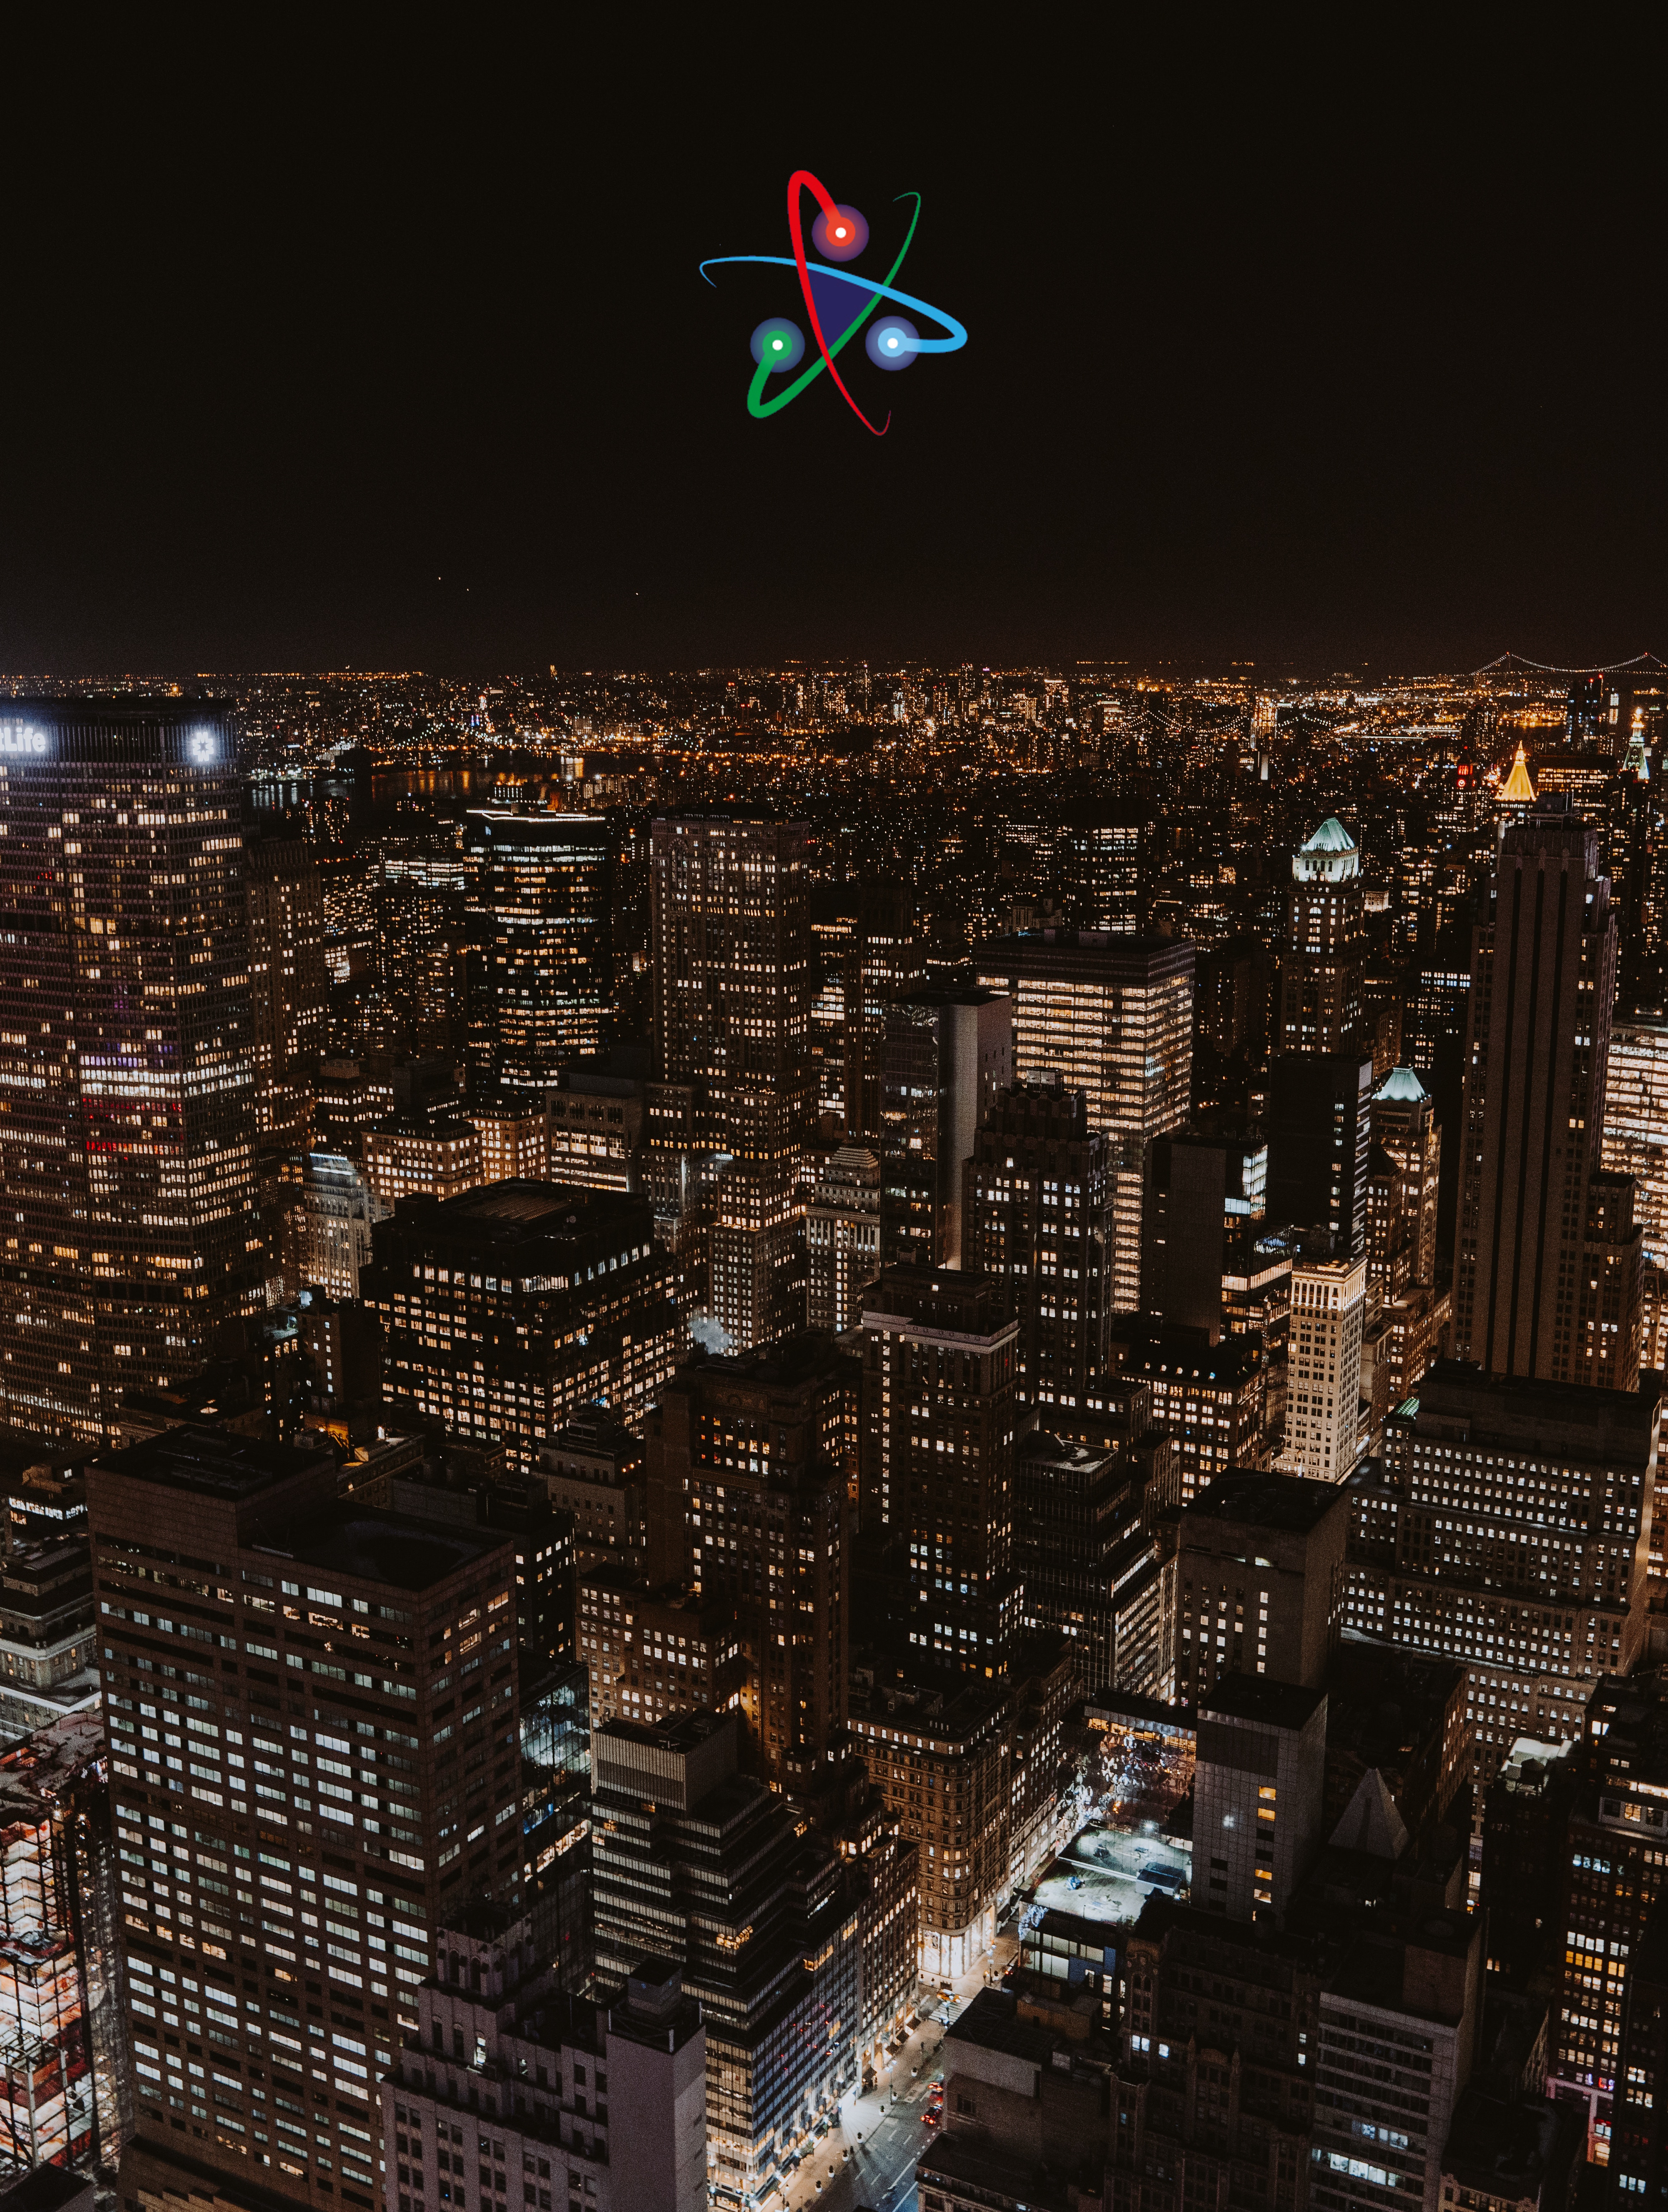
\includegraphics[height=\paperheight]{background}};
\end{tikzpicture}
\endgroup

%----------------------------------------------------------------------------------------
%	COPYRIGHT PAGE
%----------------------------------------------------------------------------------------
\newpage
~\vfill
\thispagestyle{empty}

\noindent Copyright \copyright\ 2018 Ripa Founder Team\\ % Copyright notice

\noindent \textsc{Pubblicato da Ripa Founder Team}\\ % Publisher

\noindent \textsc{www.ripaex.io}\\ % URL

\noindent Materiale protetto dalla Licenza MIT (di seguito la ``Licenza''). Non dovrai usare questo file eccetto in conformità con la Licenza. Puoi ottenere una copia della Licenza a \url{https://opensource.org/licenses/MIT}. A meno che non sia richiesto dalla lagislazione applicata o concordato via scritto, il software distribuito con la Licenza è distribuito \textsc{``così com'è'' senza garanzie di alcun tipo}, esplicite o implicite. Fate riferimento alla Licenza per il linguaggio specifico che governa i permessi e le limitazione indicati dalla Licenza.\\ 

\noindent \textit{Prima pubblicazione, Marzo 2018 - versione 1.0}\\ % Printing/edition date

\noindent \textit{RipaEx P.IVA 04927110264 - Treviso (TV) - Italia} % Printing/edition date

% \begingroup
% \section{Abstract}\index{Abstract}
% \thispagestyle{empty}
% \addcontentsline{toc}{chapter}{\textcolor{trolleygrey}{Abstract}}
\pagestyle{empty} % No headers
\usechapterimagefalse % If you don't want to include a chapter image, use this to toggle images off - it can be enabled later with \usechapterimagetrue
\chapter{Abstract}

\textbf{Ripa Exchange è un exchange ibrido-decentralizzato con il focus di abbassare il livello di ingresso per aprire 
nuove piattaforme di exchange ed al contempo offrire ai traders un ambiente sicuro ed efficiente per eseguire operazioni di 
trading giornaliere.}\\

Il Team di RipaEx crede che, indipendentemente dagli sviluppi nel mondo delle criptomonete, è oggigiorno costoso per aprire,
gestire, e trovare fiducia nelle proprie operazioni di cambiavaluta virtuale non solo per le risorse richieste per avviare
una piattaforma di scambio affidabile ma soprattutto per sviluppare la piattaforma in sè e trovare la liquidità 
necessaria per generare profitto nei primi 5 anni di attività.\\

Azione è richiesta ed azione è richiesta adesso. Gli utenti sono frustrati da exchange inaffidabili che chiudono scappando con i 
fondi, vengono hackerati oppure non sostengono il carico giornaliero di una'industria crescente come questa è.
Nonostante l'impegno degli imprenditori di exchange per offrire piattaforme di cambio valuta efficienti, affidabili e 
semplici da utilizzare i fondi necessari per costruire queste piattaforme sono nella fascia di 250-300 mila euro senza includere
il costo del personale per offrire supporto di livello platino agli utenti finali, l'infrastruttura di gestione, e costi giornalieri
dell'attività. Tali costi vengono sostenuti per avere una piattaforma di medio livello che per metterla in funzione ci si lega 
ad unica via con una software house per sviluppi futuri.\\

É obbiettivo di questo progetto di sviluppare una piattaforma di cambiavaluta virtuale Open Source, efficiente, affidabile ed 
offrire liquidità\footnote{Grazie alla tecnologia RLSP (Ripa Liquidity Service Provider)} all'exchange così creato dal \textbf{primo}
giorno di attività in modo tale che gli imprenditori in questo settore possono focalizzarsi nel pubblicizzare la propria piattaforma,
offrire supporto tecnico di livello platino ai propri utenti e soddisfare tutte le eterogenee legislazioni nell'industria delle valute virtuali.
Mentre vogliamo che l'esperienza di trading per l'utente finale sia la migliore possibile offrendo un ambiente di trading sicuro ed affidabile.\\
\usechapterimagetrue
% \endgroup

%----------------------------------------------------------------------------------------
%	TABLE OF CONTENTS
%----------------------------------------------------------------------------------------
\chapterimage{chapter_head_1_Beijing.jpg} % Table of contents heading image
\renewcommand*\contentsname{Indice dei Contenuti}
\tableofcontents % Print the table of contents itself
\addcontentsline{toc}{chapter}{\textcolor{trolleygrey}{Indice dei Contenuti}}
\cleardoublepage % Forces the first chapter to start on an odd page so it's on the right
\pagestyle{fancy} % Print headers again
%----------------------------------------------------------------------------------------
%	PART
%----------------------------------------------------------------------------------------


%\part{Part One}

%----------------------------------------------------------------------------------------
%	CHAPTER 2: Introduction
%----------------------------------------------------------------------------------------
%----------------------------------------------------------------------------------------
%	CHAPTER 2: Introduction
%----------------------------------------------------------------------------------------

\chapterimage{chapter_head_2_London.jpg} % Chapter heading image
\chapter{Introduzione}
Il livello di accesso all'industria delle valute virtuali è piuttosto elevato da un punto di vista tecnico per l'utente medio, 
ed ha un livello di accesso economicamente elevato per l'imprenditore che vuole avviare un'attività in questo campo, valore dato 
dall'acquisto del codice sorgente dell'exchange di criptovalute, dal reclutamento di personale che gestirà l'infrastruttura informatica,
per reclutare operatori di supporto tecnico, per sottostare alle leggi nazionali ed internazionali in materia di AML/KYC, per avere liquidità
dal primo giorno di avvio delle operazioni di cambio. Con questo progetto, Ripa Exchange, vuole abbassare questo livello di ingresso 
perchè \textbf{gestire un exchange è DIFFICILE} ed il Team RipaEx vuole che il lettore e futuro imprenditore nel campo delle valute
virtuali si concentri su cose veramente importanti non cavilli burocratici che l'industria richiede perchè TU vuoi avviare un'attività
in questo campo e tu necessiti del codice sorgente per avviarla, codice sorgente che deve essere concesso gratuitamente alla tua attività.

Per rafforzare questo principio economico il punto è che per avviare un exchange è richiesto un investimento esiguo dal tuo 
venture capital di riferimento e anche con un tale investimento il ritorno dei fondi investiti all'angel investor non sono garantiti
nei primi 5 anni di attività.

Per avviare un servizio professionale di cambiavaluta virtuale crediamo che il codice sorgente dell'exchange e la liquidità da offrire ai tuoi clienti
dal primo giorno di attività dovrebbero esserti forniti gratuitamente: non deve essere accettabile pagare \euro150.000,00 ad una software house
solo per avere una piattaforma che funzioni e per la quale dovete erogare altri \euro100.000,00-150.000,00 per brandizzarla, personalizzarla
per i vostri scopi legandovi in questo modo ad una singola software house che potrebbe fallire in futuro e che vi farebbe ritrovare
senza poter fare ulteriori modifiche al vostro exchange in quanto non vi hanno mai consegnato il codice sorgente della piattaforma
su cui il vostro business fa affidamento.

\textbf{Noi crediamo che tutto questo debba essere gratuito}: dobbiamo offrirti la miglior tecnologia nel mercato attuale in modo tale che tu 
possa focalizzarti sulla tua attività mentre noi ci focalizziamo in sviluppare la tecnologia per gestire la tua attività in maniera efficiente, 
sicura, responsiva e produttiva. Questo è il motivo per cui RipaEx si prefigge lo scopo di sviluppare una rete di exchange
focalizzandosi su di un'architettura che è \textit{efficiente, sicura, responsiva, compliant e personalizzabile} in modo tale che ogni exchange
nella rete può basarsi su di fondamenta solide mentre è comunque possibile modificare la singola istanza secondo le personalizzazioni 
che la compagnia che gestisce quell'istanza richiede.

Per raggiungere questo scopo abbiamo scelto di sviluppare la tecnologia Ripa Liquidity Service Provider basata su ARK - a blockchain for consumer adoption - 
il cui obbiettivo primario è incrementare l'adozione delle tecnologie blockchain agli utenti finali focalizzandosi su due aree critiche: 
\underline{Una Efficiente e Sicura Tecnologia di Base} e \underline{Servizi Reali per Gente Comune}. L'ecosistema ARK è ancora ad uno stadio
iniziale di sviluppo: la futura implementazione di ARK 2.0 permetterà di eseguire smart contract nativi sulla blockchain, che permetteranno
alla blockchain ARK di competere con la sua concorrente Ethereum da un punto di vista tecnologico. RLSP permetterà a tutti gli exchange della rete Ripa
di scambiare liquidità condividendo lo stesso libro degli ordini in base ai parametri di condivisione della singola istanza dell'exchange Ripa
configurabili nella tua area amministratore.

Il Ripa Founder Team (RFT), come presentato in ripaex.io, opera nel nome del gruppo Ripa. L'RFT è responsaile per l'uso corretto dei finanziamenti
ottenuti nella campagna di scambio token RIPA TEC come spiegato di seguito in questo documento.

Il RFT dispone che i fondi delle fasi di PreSale e RIPA TEC saranno usati esclusivamente per il finanziamento del progetto 
\emph{RipaEx} come spiegato in questo whitepaper, che saranno resi disponibili per estrazione nella piattaforma apposita resta disponibile
più tardi quest'anno tec.ripaex.io, e che dovranno risultare nella creazione di una entità legale che sarà chiamata \emph{RipaEx}. La creazione di tale 
compagnia è pianificata per il primo quadrimestre del 2019.

Fino a tale data RFT opera invece di \emph{RipaEx, una compagnia nel processo di essere incorporata}.

\section{Terminologia}\index{Terminologia}
\begin{description}
	\item[\textsc{Ripa Exchange:}] un exchange FIAT $\Leftrightarrow$ CRYPTO sviluppato partendo dal codice sorgente di Peatio \cite{peatio}
	\item[\textsc{Ripa Blockchain:}] una blockchain DPOS in cui la liquidità ed il libro mastro degli ordini sono condivisi tra tutti gli exchange della rete
	\item[\textsc{Ripa Token - XPX:}] un token crittograficamente sicuro tramite il protocollo DPOS scambiato sulla blockchain Ripa 
	\item[\textsc{RIPA:}] l'ecosistema finanziario DPOS composto da Ripa Exchange e Ripa Blockchain
	\item[\textsc{RIPAEX:}] il nome del progetto, sito web del progetto e domini del progetto
	\item[\textsc{RLSP:}] Ripa Liquidity Service Provider, un libro ordini condiviso tra gli exchange nella stessa rete Ripa
	\item[\textsc{RipaEx ICO:}] il nome del periodo di cambiavaluta a tasso fisso composto dalle fasi di PreSale e RIPA TEC	
	\item[\textsc{ARK:}] una piattaforma per l'adozione consumer di tecnologie blockchain \cite{ark}
	\item[\textsc{ACES:}] Ark Contract Execution Services \cite{aces} fornisce semplici protocolli e strumenti per costruire robusti
	mercati di scambio tra blockchain basati sulla tecnologia ARK SmartBridge
	\item[\textsc{``,'' o ``.'':}] la notazione italiana per virgola decimale e punti di migliaia è stata scelta per la stesura di questo 
	whitepaper: detto questo “,” rappresenta un punto decimale e “.” rappresenta la separazione tra migliaia e multipli di migliaia 
\end{description}

%\pagebreak
\section{Roadmap}
Saranno percorse essenzialmente quattro fasi del progetto RipaEx:
\tcbset{roadmapBox/.style={colback=yellow!10!white,colframe=azure(colorwheel),
equal height group=nobefaf,width=(\linewidth-1pt), height from=4cm to 8cm, nobeforeafter,
	center title,
	valign=top, halign=left}}
\begin{center}
\begin{tcolorbox}[roadmapBox,
	title=\textbf{\textsc{Finanziamneto del progetto: XPX presale e RIPA TEC (WP2)}}]

	Questa fase riconosce l'esistenza di un interesse in questo sviluppo di mercato
	da un capo del Mondo all'altro in riguardo l'abbassamento del livello economico di ingresso
	per sviluppare exchange di criptovalute.
	L'obbiettivo è di eseguire la prima analisi omnicomprensiva dello stato dell'arte per fondare
	le basi delle fasi sucessive del progetto e per sviluppare il primo prototipo
	funzionante di un exchange centralizzato con il codice di Peatio.\\
	\vspace{1cm}
	\centering\textbf{\textsc{Prevista fine della fase: Gennaio 2019}}.
\end{tcolorbox}
\resizebox{0.05\textwidth}{26pt}{$\Downarrow$}
\begin{tcolorbox}[roadmapBox,
	title=\textbf{\textsc{Apertura del primo exchange e sviluppo di strumenti e risorse (WP3)}}]

	La seconda fase prende i risultati della prima e sviluppa da qui
	una serie di strumenti e risorse che offrono guida concisa ed omnicomprensiva per 
	i player senza considerare lo Stato di incorporazione/sviluppo del progetto. Con la prima
	istanza di Ripa Exchange in esecuzione/aperta al pubblico i primi contatti con altri player economici
	nell'industria delle valute virtuali possono essere presi.\\
	\vspace{1cm}
	\centering\textbf{\textsc{Prevista fine della fase: Giugno 2019}}.
\end{tcolorbox}
\resizebox{0.05\textwidth}{26pt}{$\Downarrow$}
\begin{tcolorbox}[roadmapBox,
	title=\textbf{\textsc{Esecuzione, diffusione (WP 7/8) e Coordinamento del Progetto (WP1)}}]

	Durante tutta la durata del progetto,
	attività di diffusione (WP 7/8) sono eseguite nelle quali i risultati dei singoli
	pacchetti di lavoro individuali sono consegnati ai relativi gruppi obbiettivo inclusi
	partners del progetto, investitori RipaEx, manager di exchange, partner bancari come anche
	tutti gli altri gruppi obbiettivo rilevanti al progetto RipaEx in esecuzione.
	Questa fase copre una vasta scala di tecniche di diffusione, da libri stampati ed 
	elettronici, a workshop e sessioni di training, hackatons, tutti aventi 
	come obbiettivo di definire standard per la comunicazione tra exchange gestiti da entità 
	pubbliche e private nell'industria delle valute virtuali.
	Un pacchetto di lavoro globale riguardante la gestione del progetto dall'inizio alla fine, 
	assicurando coordinazione adeguata, quality assurance e controllo del budget (WP1).
\end{tcolorbox}
\resizebox{0.05\textwidth}{26pt}{$\Downarrow$}
\begin{tcolorbox}[roadmapBox,
	title=\textbf{\textsc{Sviluppo di un exchange ibrido-decentralizzato (WP 4-6)}}]

	Usando gli strumenti e le risorse sviluppate in WP3, il pacchetto di lavoro 4-6
	si focalizza di mettere in pratica la conoscenza acquisita e gli strumenti. I tre
	pacchetti di lavoro riflettono tre punti focali (e gruppi target) nel network di 
	exchange creato per installare demo di successo su scala locale, nazionale ed internazionale:
	l'incorporazione di istanze di Ripa Exchange locali (WP4), analisi tecnica della tecnologia
	Ripa Liquidity Service Provider (WP5), e primo MVP dell'exchange ibrido decentralizzato (WP6).
	La fase demo dal cuore dell'azione RipaEx; WP 2 e 3 focalizzano in produrre consegne (ad esempio
	strumenti) che abilitano attività di produzione demo efficienti e di successo.\\
	\vspace{1cm}
	\centering\textbf{\textsc{Prevista fine della fase: Gennaio 2021}}.
\end{tcolorbox}
\end{center}

\section{RipaEx Partners - RipaEx Governance}\index{RipaEx Partners - RipaEx Governance}
La maggior parte dei parnter sono imprenditori nell'industria delle valute virtuali, tuttavia
un Istituto di Ricerca ed Organizzazioni Finanziari sono anche presenti. I partner sono:
\begin{itemize}
	\item \textbf{Coordinatore}: RipaEx SCIC 
	\item \textbf{CoBeneficiari}: Ripa Exchange Ltd \todo{TODO: AGGIUNGERE PARTNER RIPAEX}
\end{itemize}

\subsection{RipaEx Governance}\index{RipaEx Governance}
La creazione di nuovi exchange nella rete Ripa, il rilascio dei fondi dell'RCF per la creazione di nuovi exchange saranno decise
su votazione maggioritaria dei delegati della rete Ripa. Le modifiche del singolo exchange, invece, saranno appannaggio 
esclusivo della compagia che gestisce la singola istanza dell'exchange.

Il progetto RipaEx si incorporerà come società di interesse collettivo per profitto appena la rete Ripa sarà stabile, mentre Ripa Exchange Ltd
società a gestione della prima istanza di exchange in esecuzione sarà incorporata come compagnia privata nel primo quarto
del 2019.

\section{Sommario del Progetto}
\begin{enumerate}
	\item \textbf{\textsc{cosa}}: RipaEx è un progetto per facilitare la presa di standard per condividere liquidità tra mercati di asset
	criptosicuri (crypto asset marketplace).
	L'obbiettio di RipaEx è la promozione di codice sorgente condiviso per portafogli ed exchange nell'industria delle valute
	virtuali: è obbiettivo di questo documento di riferimento di dare informazioni dettagliate per futuri
	sviluppatori di exchange oppure futuri imprenditori in questo campo, per abilitare processi di decision-making corretti e per 
	assicurare il successo dei loro progetti proposti.
	Il progetto RipaEx si prefigge l'obbiettivo di analizzare il potenziale reale di applicazione nel Paese scelto 
	di una rete di exchange e la sua posizione nel mercato.
	\item \textbf{\textsc{cosa}}: gli asset crittograficamente sicuri (aka: ``crypto assets'') sono un'alternativa agli asset emessi dalle borse
	valori dei vari Paesi che ne possiedono una. Anche se, tuttavia, molte borse valori mondiali danno la possibilità ai loro 
	utenti di verificare e gestire gli asset in loro possesso il processo non è sempre trasparente e/o semplice e questo è il motivo 
	per cui a partire dal 2009 \cite{bitcoin} un nuovo tipo di asset (verificabile dalla comunità) è stato implementato
	per dare a piccoli, medi e grandi investitori completa trasparenza nella gestione dei loro asset di investimento.
	\item \textbf{\textsc{quanto}}: recenti sviluppo a livello dell'Unione Europea e globalmente stanno trasformando sia come le valute virtuali
	sono trattate sia il modo in cui le ICO (Initial Coin Offering) sono legislate. Questi sviluppi combinati hanno messo
	l'uso e la produzione di valute virtuali in una luce favorevole in costante ascesa. \\
	In Ottobre 2015 la Corte Europea di Giustiza ha sentenziato che bitcoin ed altre valute virtuali sono esenti dalla tassazione IVA. \\
	In Luglio 2016 la Commissione Europea ha adottato proposal per ammendare la legislazione vigente 4th Anti-Money Laundering Directive (4AMLD) 
	che introduca le figure degli exchange di valute virtuali ed offritori di wallet all'interno del framework europeo di adeguata verifica
	dell'utente ed antiriciclaggio \cite{EUAMLCrypto}.\\
	In Febbraio 2018 la Commissione Europea lancia l'Osservatorio EU sulle Blockchain (EU Blockchain Observatory and Forum) \cite{EUBOaF} 
	per osservare gli sviluppi chiave nella tecnologia blockchain, promuovere attori europei e rafforzare l'ingaggio europeo con
	diversi stakeholders coinvolti in attività correlate alla blockchain.
	\item \textbf{\textsc{perchè}}: c'è ancora poca regolamentazione sulle ICO e solo gli Stati Uniti d'America al momento
	hanno scritto una legislazione definendo i token delle ICO come securities \cite{SECICO}.
	\item \textbf{\textsc{chi}}: i risultati delle indagini di mercato indicano che il medio tech savvy dai 18 ai 45 anni di età è
	l'utente medio delle valute virtuali tuttavia compagnie in finanza stanno anche comincianto ad inserire schemi di 
	valute virtuali all'interno dei loro portafogli specialmente dalla presentazione del contratto bitcoin futures 
	da parte del Gruppo CME Group Inc. nella borsa valori di Chicago lo scorso 18 Dicembre 2017.
	\item \textbf{\textsc{quanto}}: la capitalizzazione di mercato totale dell'industria delle valute virtuali è stata stimata attorno
	ai 317 miliardi di USD \footnote{Dati Coinmarketcap Aprile 2018}
	ed è prevista la crecita a 5.000 miliardi di USD nel prossimo timeframe di 10 anni \cite{cryptoMCTenYears}.
	\item \textbf{\textsc{dove}}: autorità locali stanno lavorando con i Governi Nazionali per essere certi che gli exchangers sul 
	territorio nazionale di riferimento seguono le procedure nazionali ed internazionali di AML/KYC.
	Venture Capital ed Angel Investors stanno cominciando a rilasciare soluzioni di finanziamento a start-up nell'industria delle
	valute virtuali - FinTech in tutto il mondo, dall'America all'Asia passando per l'Europa ed alcuni Paesi
	stanno avviando schemi di valuta virtuale statali per testare lo scambio di beni e servizi sulle tecnologie a libro 
	mastro condiviso (DLTs - Distributed Ledger Technologies) \cite{petro}.
	\item \textbf{\textsc{quanto costa}}: il costo medio per avviare il proprio crypto assets marketplace è attorno a \euro 150.000,00, 
	al pagamento di tale somma avrete unicamente un'istanza in esecuzione della vostra piattaforma di cambio: al suddetto prezzo dovete aggiungere i costi
	di personalizzazione della piattaforma prima del lancio ed in futuro, pubblicizzazione della piattaforma, costo di gestione dei server, 
	amministratori di rete, operatori del centro di supporto e costo del dipartimento legale per seguire le leggi AML/KYC dello Stato
	in cui avete deciso di incorporare il vostro exchange e per gestire l'amministrazione della compagnia dietro di esso.\\
	\textbf{Questi costi nascosti sono la ragione per cui noi di RipaEx riteniamo che possedere il codice sorgente del proprio exchange è il miglior
	modo per avviare e mantenere un'attività in questa industria}.
	\item \textbf{\textsc{come}}: il problema principale nell'eseguire un'operazione di cambio FIAT $\Leftrightarrow$ CRYPTO è di trovare partner bancari affidabili
	e nel seguire le differenti procedure AML/KYC del Paese o dei paesi di incorporazione.
	\item \textbf{\textsc{cosa}}: le operazioni di cambio valuta virtuale classiche sono le seguenti:
		\begin{itemize}
			\item \textbf{scambio ad una-via}: nella quale un'applicazione centralizzata ha tutta la liqudità da offrire ai potenziali utenti
			\item \textbf{scambio a due-vie}: nella quale un exchange centralizzato o decentralizzato accoppia richiesta di vendita con richiesta di aquisto degli utenti
		\end{itemize}
		Dalla classificazione data sopra una ulteriore sotto-classificazione è d'obbligo:
		\begin{itemize}
			\item \textbf{scambio FIAT $\Leftrightarrow$ CRYPTO}: nella quale lo scambio avviene tra valuta FIAT\footnote{Valute emesse dalle banche centrali: EUR, USD, GBP, JPY, altre...}
			e valuta virtuale
			\item \textbf{scambio CRYPTO $\Leftrightarrow$ CRYPTO}: nella quale lo scambio avviene tra valuta virtuale e valuta virtuale
		\end{itemize}
	Dalle quattro classificazioni sopra si può costruire una matrice con quattro possibili configurazioni per sviluppare la piattaforma di cambia valuta virtuale
	che preferite.
	\begin{tcbraster}[raster columns=3,raster rows=1,raster height=0.8cm,
		valign=center, halign=center,
		enhanced,size=small,sharp corners,colframe=azure(colorwheel),coltext=white,
		colback=azure(colorwheel),fit algorithm=hybrid* ]
		\tcboxfit{}
		\tcboxfit{\textbf{una-via}}
		\tcboxfit{\textbf{due-vie}}
	\end{tcbraster}
	\begin{tcbraster}[raster columns=3,raster rows=2,raster height=5cm,
		valign=center, halign=center,
		enhanced,size=small,sharp corners,colframe=silver,coltext=black,
		colback=silver,fit algorithm=hybrid* ]
		\tcboxfit{\textsc{\textbf{FIAT $\Leftrightarrow$ CRYPTO}}}
		\tcboxfit{\tcbfontsize{0.8} applicazione di acquisto veloce}
		\tcboxfit{\tcbfontsize{0.8} exchange con partnership bancaria}
	
		\tcboxfit{\textsc{\textbf{CRYPTO $\Leftrightarrow$ CRYPTO}}}
		\tcboxfit{\tcbfontsize{0.8} applicazione di scambio veloce}
		\tcboxfit{\tcbfontsize{0.8} exchange senza partnership bancaria}
	\end{tcbraster}	

	\item \textbf{\textsc{con cosa}}: le specifiche da guardare quando scegliere la propria piattaforma di exchange sono le seguenti: 
		\begin{enumerate}[label*=\arabic*.]
			\item \textbf{Codice}: Open Source, Closed Source oppure soluzione ibrida
			\item \textbf{Modularità}: separazione tra l'engine di cambio (engine di accoppiamento ordini), la UI e l'anagrafica utenti
			\item \textbf{Responsività della UI}: la UI deve essere responsiva su tutti i device (desktop e mobile)
			\item \textbf{Conformità}: con gli standard industriali correnti e con la legislazione vigente
			\item \textbf{Personalizzazione}: dell'engine di cambio, delle valute da offrire, della UI e di altri aspetti della piattaforma di cambio
			\item \textbf{Sicurezza} dei fondi nell'exchange: possibilità di configurare il salvataggio dei fondi in cold wallet e hot wallet
			\item \textbf{Trasparenza} dei fondi: proof of solvency dell'exchange
			\item \textbf{Multi-Accounts trading}: possibilità di configurare facilmente nuovi mercati da offrire agli utenti
			\item \textbf{Multi-Accounts users}: possibilià di loggarsi nella piattaforma tramite Google, Facebook, Twitter, e conformità
			con gli standard della FIDO Alliance per le credenziali personali
		\end{enumerate}	
	\textbf{Queste non sono solo decisioni tecniche da prendere ma anche economiche} specialmente il possesso o meno del codice sorgente della propria 
	piattaforma	crypto asset marketplace per permettere le future personalizzazioni del proprio exchange in maniera indipendente invece di affidarsi
	ad una singola software house che esegua le personalizzazioni per voi.
	\item \textbf{\textsc{come}}: possibili operazioni per trovare nuovi utenti per le vostre operazioni di cambia valuta virtuale sono:
	campagne di marketing ``ad hoc'', funzionalità innovative nell'industria, livelli di tassazione del trading basati sulla quantità, 
	bonus di registrazione e per quantità di scambiato giornaliero/settimanale/mensile, marketing affiliato per gli utenti che portano
	amici a scambiare nell'exchange.
	\item \textbf{\textsc{come}}: per incorporare una crypto asset marketplace un progetto deve tenere in considerazione la seguente legislazione:
		\begin{itemize}
			\item \textbf{AML/KYC}: \textit{Fourth Anti-Money Laundering Directive} se l'attività viene avviata nell'Unione Europea \cite{4AMLD} 
			oppure la legge AML/KYC di riferimento nel Paese di incorporazione (ad esempio \textit{Intelligence Reform \& Terrorism Prevention Act of 2004}
			emessa dalla FinCEN per incorporazione negli Stati Uniti d'America).\\
			Raccomandazioni internazionali per eseguire verifiche AML/CFT sono data dalla Financial Action Task Force on Money Laundering \cite{FATF}.
			\item \textbf{Licenza di Pagamento}: l'attività decisamente più ardua in riguardo alla legittimazione delle operazioni di cambio FIAT $\Leftrightarrow$ CRYPTO
			è l'ottenimento di una \textit{Licenza PSD} \cite{PSD}.
			La licenza PSD seguen la Direttiva del Concilio Europeo 2007/64/EC ed è applicata in ogni Paese attraverso le sue leggi nazionali.
			Il costo di una licenza PSD può variare da centinaia di migliaia di euro ad un ordine di grandezza superiore al seconda del volume di affari.
		\end{itemize}
	\item \textbf{\textsc{chi}}: la natura dell'attività in considerazione del progetto RipaEx 
	(una rete di piccoli exchange FIAT $\Leftrightarrow$ CRYPTO)
	implica che ogni exchange debba avere uno staff di 7-8 persone: N.2 sviluppatori, N.1 operatore di rete/sicurezza, 
	N.1 commerciale amministrativo, N.2 operatori di supporto tecnico, N.1 legale e consigliere sulla tassazione. \\
	Il turnover di una tale compagnia tuttavia, considerato l'alto valore aggiunto del prodotto scambiato, e possibile che raggiunga cifre
	superiori ad \euro 350.000 annui e possibilmente di un'ordine di grandezza superiore. Un'attività di questa dimensione
	suggerisce automaticamente le possibili forme societarie: una ditta individuale, una società a responsabilità limitata,
	una società non-profit o attività sociale, una cooperativa gestita dagli amministratori delegati dei vari exchange.
	Le Agenzie Finanziarie sono attori fondamentali nell'indicare questa scelta, tuttavia la tipologia di attività da
	incorporare dipende dallo status legale che si vuole dare alla stessa e questo varia da Paese a Paese.		
	\item \textbf{\textsc{come}}: una risorsa di fondi per una marketplace di dimensioni piccole-medie può essere: prestito bancario,
	prestito privato a basso interesse, credito commerciale, equity finanziario, venture capital di business angels. Avendo un
	business plan consolidato e garanzie finanziarie adeguate sono elementi chiave nell'assicurarsi i finanziamenti necessari
	allo sviluppo che si vuole eseguire. Il Fondo Europeo di Investimento (EIF) della Banca di Investimento Europea (EIB)
	offre supporto nella forma di garanzia per le SME (piccole e medie imprese).
	\item \textbf{\textsc{chi}}: gli argomenti per l'incorporazione di un crypto asset marketplace sono la libertà finanziaria, la
	decentralizzazione delle operazioni di trasferimento del valore ed il reale possesso del proprio denaro.
	Ci sono altri benefici, ben documentati, come pagamenti veloci, guadagno a lungo termine dato da un'economia deflazionaria, previsione
	delle depressioni economiche come quella del 2008, ma soprattutto le valute virtuali sono l'unico competitor diretto alle operazioni
	di trasferimento del valore centralizzate eseguite dalle banche centrali.
	\item \textbf{\textsc{perchè}}: c'è consenso in letteratura che l'uso delle valute virtuali invece delle valute fiat permette un livello di
	libertà finanziaria maggiore specialmente perchè queste tecnologie di trasferimento valore rientrano nella scuola
	di economia Austriaca \cite{austrianTheory} secondo molte fonti \cite{misesItalia} anche se tuttavia bitcoin dà il meglio come
	mezzo di scambio e mancherebbe della stabilità di tasso di cambio che la renderebbero una riserva di valore accettabile.
	\item \textbf{\textsc{perchè}}: benefici delle tecnologie di valuta virtuale come bitcoin sono in una economia deflazionistica,
	in un'emissione limitata di valuta, in trasferimenti di valore pressochè istantanei e senza barriere statali, in 
	relativo anonimato e nella separazione tra entità che producono la moneta (miner) ed entità che definiscono la teoria monetaria
	alla base della stessa (sviluppatori).
	\item \textbf{\textsc{come}}: securizzare asset sulla blockchain significa semplicisticamente eseguire le tre operazioni
		\begin{enumerate}[label*=\arabic*.]
			\item \textbf{Generazione di una chiave privata casuale}
			\item \textbf{Conversione della chiave privata generata in (1) in una chiave pubblica}: un protocollo comune per la conversione
			in questa industria è l'algoritmo ECDSA
			\item \textbf{Conversione della chiave pubblica generata in (2) in un indirizzo di valuta}: protocolli comuni per eseguire questa
			conversione sono le funzioni hash SHA-256, Base58 encoding, Base32 encoding
		\end{enumerate}
	A questo punto qualsiasi valore inviato all'indirizzo generato in (3) è garantito dalla doppia spesa nella blockchain scelta ed accessibile
	solo dal possessore della chiave privata generata in (1).
	\item \textbf{\textsc{dove}}: due fattori critici che interessando l'industria delle valute virtuali sono la concorrenza bancaria ed il 
	banning a livello statale. Anche se l'armonizzazione delle leggi europee in materia sarà di beneficio all'industria sia in termini di 
	tassazione sia in termini di garanzia per l'utilizzatore finale, al momento questo ancora non avviene. Ogni Paese su scala mondiale 
	ha la propria legislazione in materia ed i propri regimi di tassazione per tutte le operazioni di cambiavaluta virtuale,
	il banning statale invece va da livelli	di permissività totale come nell'Unione Europea al banning totale con 
	imprigionamento come in Bangladesh \cite{bitcoinLegality}. 
	\item \textbf{\textsc{dove}}: i paesi asiatici della Corea del Sud, Cina e Giappone sono sempre stati leader nell'industria delle valute virtuali
	negli ultimi 9 anni con un approccio proattivo in materia di tassazione. All'inizio del 2017 in Giappone il bitcoin è stato 
	dichiarato legal tender tuttavia in Cina recentemente sono state dichiarate illegali tutte le operazioni di cambiavaluta virtuale ed ICO 
	e gli exchange nel Paese asiatico stanno cessando le loro attività di cambio. 
	\item \textbf{\textsc{dove}}: qualsiasi valutazione del mercato locale dovrebbe comprendere: numero di potenziali utenti, tipo di exchange da 
	incorporare (FIAT $\Leftrightarrow$ CRYPTO oppure CRYPTO $\Leftrightarrow$ CRYPTO), tipi di protocolli da integrare (POW, DPOS, Masternode, altri...), 
	tipi di servizi da offrire (trading, trading avanzato, processore di pagamento, altri...), se l'exchange incorporato è di tipologia
	FIAT $\Leftrightarrow$ CRYPTO numero e tipologia di processori di pagamento accettati (PayPal, OKPAy, MoneyPolo, altri...), numero di exchange
	simili nella regione di incorporazione. 
	\item \textbf{\textsc{chi}}: ci sono numerose opzioni per offrire una polizza assicurativa sui fondi degli utilizzatori finali (Customer Protection):
	creare comprensione tra gli utenti che il possesso delle chiavi private dei fondi mette loro in \textbf{posizione di responsabilità} 
	nei confronti di un'eventuale perdita dei fondi, in quanto nessuno può recuperare le chiavi private una volta che sono perse. 
	Creare comprensione negli utenti per non lasciare i fondi negli exchange ("\textit{Be Your own Bank!!}"), lasciandogli scegliere a quale
	exchange del mercato affidarsi.
	\item \textbf{\textsc{chi}}: mentre è decisamente costoso assicurare la valuta e le operazioni di trasmissione del valore, esempi di customer protection
	in questa industria sono: la piattaforma Kraken ha recentemente permesso agli utenti Mt. Gox di richiedere rimborso tramite
	la loro piattaforma, l'exchange BitFinex ha emesso token BFX per ripagare i propri utenti della perdita di 120.000 bitcoin (pari a circa \$72.000.000
	all'epoca dell'hacking) dovuti al cambio del livello di sicurezza dell'exchange stesso, Ethereum ha eseguito uno fork al blocco 1920000
	per ovviare ad un bug nel codice della Decentralized Autonomous Organization che ha permesso la sottrazione di \$50.000.000 di ETH dallo smart contract
	di The DAO, altri casi di hacking...
	\item \textbf{\textsc{Raccomandazioni finali/conformità legislativa}}: se intendete incorporare un exchange 
	FIAT $\Leftrightarrow$ CRYPTO dovete focalizzarvi in prima istanza nella conformità legislativa in materia 
	di AML/KYC nel Paese di incorporazione, le fondazioni
	bitcoin locali possono aiutarvi in focalizzare le vostre operazioni di cambio basate sugli interessi degli utilizzatori finali 
	nel Paese di incorporazione, promuovendo ambienti \textit{cryptocurrency friendly} nell'area di interesse.
\end{enumerate}


%----------------------------------------------------------------------------------------
%	CHAPTER 3: Ripa Exchange
%----------------------------------------------------------------------------------------
%----------------------------------------------------------------------------------------
%	CHAPTER 3: Ripa Exchange
%----------------------------------------------------------------------------------------

\chapterimage{chapter_head_3_Singapore.jpg} % Chapter heading image

\chapter{The Ripa Exchange}
Ripa Exchange is an crypto asset (fiat money or cryptocurrency or something) marketplace, following the latest 
industry standards and resting in the principles of ``\textit{open source, secure and efficient}''. Ripa Exchange
aims to serve a platform for crypto-currency enthusiasts by providing a safe, secure, UI responsive, customizable 
and easy to use exchange that embraces open source principles and public trust.\\\\
Ripa Exchange is implemented with the Rails framework and other cutting-edge technology and will be migrated to an
hybrid-decentralized exchange where all exchanges in the Ripa network will share liquidity thanks to RLSP technology.

\section{Mission}
\begin{quotation}
	``\textit{Our mission is to build the world best open source crypto asset marketplace with a high performance trading engine 
	and safety which can be trusted and enjoyed by users. Additionally we want to move the crypto currency exchange technology 
	forward by providing support and add new features. We are helping people to build easy their own exchange around the world.}''
\end{quotation}

Help is greatly appreciated, feel free to submit pull-requests or open issues in our \href{https://github.com/RipaEx}{GitHub repositories}.

\section{Features}
A free, transparent and internationalized open source crypto currency exchange.

\tcbset{featureBox/.style={colback=yellow!10!white,colframe=white!20!black,
equal height group=nobefaf,width=(\linewidth-1pt)/3, height=5.0cm, nobeforeafter,
	center title,
	valign=top, halign=left}}
\begin{tcolorbox}[featureBox,
	title=\textsc{Open Source} \faCircleONotch]

	\small	All source code are fully released under the terms of the MIT License.\\\vspace{5mm}
	\tiny Ripa Exchange is a customizable cryptocurrency exchange solution architecture enables easy connection to KYC/AML, 
	authentication, ETL/reporting, and other services.
\end{tcolorbox}
\begin{tcolorbox}[featureBox,
	title=\textsc{Compliant} \faCheck]

	\small	International KYC/AML standards.\\\vspace{5mm}
	\tiny Ripa Exchange KYC efficiently submits and exchanges KYC information 
	to meet the banking supervisory standards and comply with Customer Due Diligence (CDD) requirements.
\end{tcolorbox}
\begin{tcolorbox}[featureBox,
	title=\textsc{Transparent \& Configurable} \faCogs]

	\small	Customize in your own way\\\vspace{5mm}
	\tiny Major functions have been embedded in the source code – neat registration and log-in interface, 
	personalized deposit and withdraw procedure, best match of bid and ask, etc. These functions are comprehensive 
	and are ready to use with no extra work needed. 
\end{tcolorbox}

\begin{tcolorbox}[featureBox,
	title=\textsc{Internationalization} \faLanguage]

	\small	All users are able to view Ripa Exchange in a language to their best convenience.\\\vspace{5mm}
	\tiny Supporting many common languages, Ripa Exchange makes it easy for users to operate in their mother tongue. 
	You are encouraged to contribute to our language variety. Users will benefit from your efforts.
\end{tcolorbox}
\begin{tcolorbox}[featureBox,
	title=\textsc{Proof of Solvency} \faUsers]

	\small	Easy deployable PoS.\\\vspace{5mm}
	\tiny Ripa Exchange Proof of Solvency (PoS) allows users to verify 
	the solvency of the Ripa Exchange based cryptocurrency exchange without compromising user privacy.
\end{tcolorbox}
\begin{tcolorbox}[featureBox,
	title=\textsc{Multi-Accounts Trading} \faHandSpockO]

	\small	Easy currency configuration.\\\vspace{5mm}
	\tiny Ripa Exchange allows to create multiple accounts and trading in multiple currencies. 
	Ripa Exchange makes it is easy to trade different currencies.
\end{tcolorbox}

\begin{tcolorbox}[featureBox,
	title=\textsc{Multi-Accounts Users} \faSuitcase]

	\small	Easy account configuration.\\\vspace{5mm}
	\tiny Ripa Exchange allows to create multiple login accounts Google, Facebook, Twitter and FIDO Alliance
	login standards to secure your account.
\end{tcolorbox}
\begin{tcolorbox}[featureBox,
	title=\textsc{Enterprise Exchange} \faInstitution]

	\small	Start small, grow big.\\\vspace{5mm}
	\tiny Ripa Exchange enterprise exchange features include a high-performance matching engine, 
	scalable distributed worker threads, and SMS 2-factor authentication.
\end{tcolorbox}
\begin{tcolorbox}[featureBox,
	title=\textsc{Functional \& Intuitive} \faIntersex]

	\small	For the new trader, for the experienced trader.\\\vspace{5mm}
	\tiny Clean, user friendly registration and login interface. 
	Personalized deposit and withdraw procedure and a built-in proof-of-solvency audit.
\end{tcolorbox}

\section{Functional Analysis}
\todo{TODO: more details here}
\begin{enumerate}
	\item \textsc{Why Redis-RabbitMQ is needed}:
	\item \textsc{Why NodeJS}: 
	\item \textsc{Why Pusher}:
	\item \textsc{ER MySQL}:
	\item \textsc{Ruby folders hierarchy}:
\end{enumerate}

\section{Technology Stack}
\todo{TODO: more details here}
\begin{itemize}
	\item \textbf{\textsc{Ruby on Rails}}:
	\item \textbf{\textsc{MySQL}}: 
	\item \textbf{\textsc{Redis}}:
	\item \textbf{\textsc{RabbitMQ}}:
	\item \textbf{\textsc{NodeJS}}:
	\item \textbf{\textsc{Pusher}}:
\end{itemize}

\section{User Interface}
Ripa Exchange user interface is based on Peatio user interface a UI responsive user interface built in Ruby on Rails and 
completely separated from the exchange order engine.
Design for a customised UI are in place to offer to Ripa Exchange users the best experience on all devices: here you can find
some screenshots of the current exchange interface design.

\subsection{End-User Interface}
Following some screenshot of the end-user Ripa Exchange-Peatio interface: 
\textcolor{darkred}{those screenshots are a work in progress and they may not represents the user interface of the final product}
\begin{center}
	\includegraphics[width=\textwidth*2/3,height=\textheight,keepaspectratio]{RE_TradingUIC}
	\captionof{figure}{Ripa Exchange trading UI}
	\includegraphics[width=\textwidth*2/3,height=\textheight,keepaspectratio]{RE_depositBTCC}
	\captionof{figure}{Ripa Exchange deposit/whitdraw}
	\includegraphics[width=\textwidth*2/3,height=\textheight,keepaspectratio]{RE_historyC}
	\captionof{figure}{Ripa Exchange order history}
	\includegraphics[width=\textwidth*2/3,height=\textheight,keepaspectratio]{RE_solvencyC}
	\captionof{figure}{Ripa Exchange solvency screen}
\end{center}

\subsection{Admin Interface}
Following some screenshot of the administrative console of Ripa Exchange-Peatio interface: 
\textcolor{darkred}{those screenshots are a work in progress and they may not rapresents the user interface of the final product}
\begin{center}
	\includegraphics[width=\textwidth*2/3,height=\textheight,keepaspectratio]{RE_adminDashboardC}
	\captionof{figure}{Ripa Exchange Admin console dashboard}
	\includegraphics[width=\textwidth*2/3,height=\textheight,keepaspectratio]{RE_adminDepositsC}
	\captionof{figure}{Ripa Exchange Admin console deposit screen}
	\includegraphics[width=\textwidth*2/3,height=\textheight,keepaspectratio]{RE_adminWithdrawsC}
	\captionof{figure}{Ripa Exchange Admin console whitdraw screen}
	\includegraphics[width=\textwidth*2/3,height=\textheight,keepaspectratio]{RE_adminUserInfo1C}
	\captionof{figure}{Ripa Exchange Admin user info screen}
	\includegraphics[width=\textwidth*2/3,height=\textheight,keepaspectratio]{RE_adminVerifyAccountC}
	\captionof{figure}{Ripa Exchange Admin verify account screen}
\end{center}

\section{Features at Launch}
At the first working Ripa Exchange instance opening the following features will be functioning:
\begin{itemize}
	\item \textsc{CRYPTO $\Leftrightarrow$ CRYPTO}:
	\item \textsc{OAuth}: Facebook, Google, Twitter
	\item \textsc{FIDO}: login with FIDO Alliance standards
	\item \textsc{Protocols}: POW, DPOS, Masternode, tether, ERC20
	\item \textsc{Currencies}: BTC, ETH, DOGE, BCH, TUSD, ARK, LISK, SHIFT, RISE, KAPU, OXY, RIPA, promising ERC20 tokens
	\item \textsc{Main Markets}: BTC, ETH, ARK
	\item \textsc{Orders Type}: market, limit
\end{itemize}

\subsection{Future Features}
Future instances of Ripa Exchange implementations will have the following features:
\begin{itemize}
	\item \textsc{E-Wallets}: OKPay, NETELLER, MoneyPolo, others...
	\item \textsc{Advanced Trading Features}: margin trading, stop loss and take profit, 
	\item \textsc{FIAT $\Leftrightarrow$ CRYPTO}
	\item \textsc{Other tools}: VISA/MasterCard, merchants tools, P2P Lending 
\end{itemize}


\section{Towards a Decentralized Exchange...}
Ripa Exchange is a centralized exchange which will be converted into an hybrid-decentralized exchange to create a network of exchanges
that share the same liquidity between each of them so you can offer liquidity from day 1 of your exchanges operations.\\

To offer the PROs of a centralized exchange like platinum customer support and FIAT exchange, with all the PROs of a 
decentralized exchange like liquidity, without the CONs of both of them, 
we need to perform an intermediate step where Ripa Exchange will be converted into an hybrid-decentralized exchange 
and during phase 3 of our project (WP4-6) we will make all the functional and technical analysis required 
to make the next step on solid ground and offer to the RipaEx community an open source, secure and efficient exchange.


%----------------------------------------------------------------------------------------
%	CHAPTER 4: Ripa Blockchain
%----------------------------------------------------------------------------------------
%----------------------------------------------------------------------------------------
%	CHAPTER 4: Ripa Blockchain
%----------------------------------------------------------------------------------------

\chapterimage{chapter_head_4_Dubai.jpg} % Chapter heading image
\chapter{The Ripa Blockchain}
\label{sec:theRipaBlockchain}
The RipaEx project will have its own blockchain called Ripa which will be run on the DPOS protocol and has the XPX 
token (\PHP symbol) running on it that will serve the five following purposes:
	\begin{enumerate}
		\item to list new cryptocurrencies on Ripa Exchanges
		\item to advertise new projects
		\item to buy RipaEx gadget on the RipaEx Store
		\item to pay for the sell of goods \& services on authorized resellers with our RipaEx POS (Point of Sale)
		\item to share liquidity between Ripa Exchanges in the same network
	\end{enumerate}

Ripa (XPX or \PHP) is a cryptocurrency derivate from ARK, Lisk, Crypti and BitShares with unique differences and improvements
for reaching the goal of shared liquidity between exchanges in the same Ripa network. This code however inherits the 
simplified interactions between ARK and other blockchain systems using DPoS as their consensus. This homogeneous codebase
allows for the potential to provide service bridges in the form of ARK-Lisk blockchain apps, along with any other additional 
systems provided by their blockchain administrators.

\vspace{5mm}
\textsc{\textbf{Ripa blockchain is an ARK fork and the use of a blockchain technology for the network of exchanges created will complete
the ripa ecosystem by permitting each exchange in the ripa network to share the same liquidity. We will always entrust ARK as our 
blockchain technology provider to merge their code into our latest features for what concerning the RIPA Blockchain}}

\vspace{5mm}

Explained the use of the Ripa Blockchain in the RipaEx ecosystem and explained the RIPA - ARK technological relations what is 
following are the specifications of the Ripa Blockchain derived/inherited from ARK.

\section{Delegated Proof of Stake Technology}
Ripa Blockchain, will inherits the Delegated Proof of Stake (DPoS) consensus system that was first introduced
by BitShares. This consensus algorithm was designed to eliminate the issues associated with Proof of Work (PoW), 
namely the centralization of computing power and the exponentially increasing waste of real world energy. While not
completely decentralized as it relies on consensus by a fixed number of elected delegates, it guarantees a better decentralization 
than Bitcoin. The consensus algorithm implementation is improved over time, evolving into an optimal consensus system.\\

The technical description of the Ripa blockchain is as follow:
\begin{enumerate}
	\item DPoS (Delegated Proof of Stake)
	\begin{itemize}
		\item 101 active forging Delegates
		\item Delegates selected by vote mechanism built into DPoS
		\item 115,000,000 XPX - Seeded Genesis Block
	\end{itemize}
	\item Multi-signature accounts
	\item Constant block reward
	\begin{itemize}
		\item 2 \PHP per block
		\item Inflation Rate (with 8s block times)
		\begin{itemize}
			\item 6.31\% for the first year
			\item 5.93\% the 2nd year
			\item 4.02\% the 10th year
		\end{itemize}
		\item 8-second block time
		\begin{itemize}
			\item Decreased block time possible with future upgrades to the core.
		\end{itemize}
		\item 25 transactions per block
		\begin{itemize}
			\item Increased via soft fork as needed.
		\end{itemize}
	\end{itemize}
	\item Routing tables
	\item SmartBridge data field for custom use and bridging blockchains (ARK Contract Execution Service)
	\item Batch transactions\footnote{Future upgrade: when ARK 2.0 will be released \label{note1}}
	\item Custom transaction fees\footnotemark[\value{footnote}]
	\item Native smart contract execution\footnote{Future upgrade: when ARK Virtual Machine will be released}
\end{enumerate}

\vspace{5mm}
\textsc{\textbf{As said Ripa blockchain is an ARK fork and we will entrust ARK as our blockchain technology provider to merge their 
code into our latest features for what concerning the RIPA Blockchain}}, features like:
\begin{itemize}
	\item \textbf{Scaling network} up to the level of major Credit Card networks with core upgrades
	\begin{itemize}
		\item Increasing the number of Forging Delegates
		\item Increasing the Block Size to include more transactions
		\item Implementation of pre-approval PBFT block concept testnet [codename:
		TwinChain]
		\item Routing tables, to minimize hops among nodes when blocks are broadcast
		\item Include forging with RIPA Uncles.	
	\end{itemize}
	\item \textbf{Two node types} is used to secure the RIPA network:
	\begin{itemize}
		\item \textbf{Relay nodes} - Nodes with full API functionality, acting as a back-end for the
		feature rich lite clients. Relay nodes do not collect any transaction fee and do
		not have the ability to Forge RIPA Blocks.
		\item \textbf{Forging nodes} - Nodes with reduced API functionality, decreasing the
		exposure to potential DDoS attacks on the RIPA Platform. Forging nodes are
		able to Forge RIPA and receive transaction fees.
	\end{itemize}
	\item \textbf{Official lite client} for network access is be provided shortly before the mainnet
	launch including desktop clients (Windows, MacOS, and Linux) and mobile clients
	(Android and iOS).
	\item \textbf{OffLine wallet creation}: the network itself does not use a Graphical User Interface by default. Any RIPA
	account can be created off-line and managed at no cost with a single device
	(computer, mobile phone, embedded ARM, IoT).
\end{itemize}

\section{Hierarchical Deterministic (HD) Wallets (BIP32)}
The structure of the public and private key generation follows the same specification
as Bitcoin. A custom implementation of BIP32 for Hierarchical Deterministic Wallets
is provided to RIPA users.

\section{Fees}
The fee for standard transactions is set at \PHP0.1 but the will be flexible in future releases of Ripa Blockchain.
At mainnet launch, a fee structure is provided out of the box to forging delegates with the following rules:
	\begin{itemize}
		\item Transaction \PHP0.1
		\item Vote \PHP1 (101 votes per transaction)
		\item Second Signature \PHP1
		\item Multi Signature \PHP1 per signature + \PHP1 per signing account
		\item Registering a delegate \PHP25.
	\end{itemize}
All fees are paid to the forging node which processes the block containing those fees.

\section{Ripa Delegates and Delegate Voting}
Any node running the core blockchain code wishing to become a forging node must
register their account within the RIPA network. The fee for this registration is set to
25 \PHP per delegate account registered.
RIPA incorporates a new DPoS voting system originally envisioned by the Crypti
Founders. The RIPA system fee is 1 \PHP per delegate vote. The voting weight of each
wallet will be split evenly between all delegates voted. For example:
\begin{itemize}
	\item If a wallet votes for one delegate, that delegate receives 100\% of the wallets
voting weight.
	\item If that wallet votes for an additional delegate, the entire vote weight is split
evenly between the two delegates at 50\%.
	\item By adding a third delegate, the voting weight splits again, and each of the
three delegates receives 33.333\% of the voting weight from that wallet.
\end{itemize}

The 101 forging nodes with the highest number of votes are eligible to Forge RIPA
blocks. This design eliminates the possibility that any single large RIPA holder or an
organization holding large percentages of RIPA are able to gain control over the
entire network by voting for all of their nodes into forging positions, thus effectively
taking complete control over that DPoS Blockchain. Votes from XPX Tokens held by
RIPA Crew may be used at RIPA Crew's discretion.

\section{Connecting Blockchains}
\subsection{ARK Bridged Blockchains (SmartBridge Technology)}
The ARK Platform does not provide direct support for sidechains or dapp databases.
Instead, a mechanism to bridge together blockchains is provided via a bridging
function built into ARK Core where any blockchain can send and receive trigger
function notices and informational data through the primary ARK network via
custom developed \textbf{SmartBridge(s)} and \textbf{Encoded Listeners}.
\begin{center}
	\includegraphics[width=\textwidth,height=\textheight,keepaspectratio]{ARKSmartBridge}
	\captionof{figure}{ARK SmartBridge Technology}
\end{center}

\subsection{A.C.E.S. - ARK Contract Execution Service}
ACES is a blockchain interoperability platform that provides simple protocols and tools for building a robust blockchain 
service marketplace.

ACES is composed mainly of the following three components:
\begin{itemize}
	\item \textbf{Listeners} ACES Listeners provide a way for all the different blockchain transaction events to be easily 
	consumed via a common REST-ful API. The API allows consumers to create subscriptions and receive blockchain events 
	in real-time using Webhook callbacks.
	\item \textbf{Services} ACES Services create and execute Service Contracts, which can be anything from uploading 
	a file to a storage blockchain, performing value transfers, creating smart contracts, executing code on 
	blockchain based computing platforms, or interacting with IoT hardware.
	\item \textbf{Marketplace Console} The ACES Marketplace Console is a consumer dashboard for searching and executing 
	service contracts listed on the Marketplace. ACES Service providers can list their service nodes using the Marketplace API.
\end{itemize}

\begin{center}
	\includegraphics[width=\textwidth,height=\textheight,keepaspectratio]{ACES}
	\captionof{figure}{ARK-BTC A.C.E.S. SmartBridge Implementation Overview}
\end{center}

\section{Ripa Liquidity Service Provider (R.L.S.P)}
Using the SmartBridge technology RipaEx will build a mechanism to share liquidity between all the exchanges in the Ripa network
by writing the single exchange orderbook in the Ripa Blockchain and by executing order matching between all exchanges in the network.

In this way you can have the benefits of a decentralized orderbook (like liquidity) with the benefits of a centralized exchange (like
platinum customer support and FIAT exchange).

\section{Ripa Community Fund}
To permits the birth of new exchanges in the Ripa network a Ripa Community Fund - RCF - is created with the following characteristics:
\begin{itemize}
	\item \textbf{Starting Principal}: the RCF will have a starting operating capital of 5\% (5,750,000 \PHP) of the genesis block
	\item \textbf{Recurring Participation}: each delegate will contribute to the RCF with 5\% of its forged XPXs
\end{itemize}
\vspace{5mm}
To obtain funds from the RCF to start your own Ripa Exchange you will submit your proposal in the official RCF section in the Ripa forum at
anytime after the first Ripa Exchange instance will be operational.


%----------------------------------------------------------------------------------------
%	CHAPTER 5: Token Sale
%----------------------------------------------------------------------------------------
%----------------------------------------------------------------------------------------
%	CHAPTER 5: Token Sale
%----------------------------------------------------------------------------------------

\chapterimage{chapter_head_5_Tokyo.jpg} % Chapter heading image
\chapter{Token Sale}
\section{Introduction}
The RipaEx XPX token sale will be separated into two phases:
	\begin{itemize}
		\item \textbf{\textsc{PreSale}}: that will run from April to June 2018
		\item \textbf{\textsc{RIPA TEC}}: that will run from July to December 2018
	\end{itemize}
\vspace{5mm}
You can easily refer to both phases PreSale and RIPA TEC as \textit{RipaEx ICO}.

\subsection{Exchange Rate \& Accepted Cryptocurrencies}
During the token sale the exchange rate for the XPX tokens will be \textbf{\PHP/\euro0.10}.\\

The following cryptocurrencies are accepted: \textbf{BTC, ETH, ARK, LISK}.\\

If you want to send us a different cryptocurrency send us your choice and we will tell you immediately if we can make 
the exchange and how to execute the operation in detail (receiving address, exchange rate, quantity)\\

\textsc{Exchange rate is Bitstamp last and is valid 60 minutes from quote}.

\subsection{Bonus for Investors and for new Users}
For all investors in the RipaEx ICO will be given \euro1,000.00 credit in trading commissions 
in the first Ripa Exchange instance running, while a bonus of \PHP1,000.00 will be given
to all new registered users during the RipaEx ICO to use at your own will.

\section{How to Invest}
\subsection{XPX Ripa Token PreSale}
Private sale of XPX tokens has \textbf{started on Monday 04/02/2018 at 00:00 GMT and will end on Sunday 07/01/2018 at 23:59 GMT}.

You can buy directly here: 
\begin{center}
	\href{https://www.ripaex.io/privsale}{\textsc{www.ripaex.io/privsale}}
\end{center}

or send us your buying inquiries on our social 
\href{https://join.slack.com/t/ripaex/shared_invite/enQtMzM4NzUwNjU4OTQ0LTY3MDJmMTdhYTNlZjJlNGUxNzM1YjUwYjgyYjZlMDJmOTg3NTIzNThmNTYyMGQ3ODBkOTRmYzk3Y2Y4MzBkOTY}{Slack},
\href{https://t.me/ripaex}{Telegram},
Facebook, Twitter or on other social networks where we are present which you can check in Section \ref{sec:social}.
For all the duration of the private sale period every exchange operation \textbf{will be executed at the exchange rate of \PHP/\euro0.0500 
until the first 5,000,000 XPX tokens} have been exchanged and will be exchanged at the rate of \PHP/\euro0.05714286 thereafter.

\subsection{RIPA TEC}
Fund-raising through the RIPA TEC platform will follow the schedule:
\begin{itemize}
	\item \textcolor{airforceblue}{\textbf{\textit{Exchange} from 07/02/2018 to 07/15/2018}}: at the rate of \PHP/\euro0.0500 (\textcolor{airforceblue}{\textbf{100\% bonus}})
	\item \textcolor{darkgoldenrod}{\textbf{\textit{Cooling-OFF} from 07/16/2018 to 07/22/2018}}: 
	at the rate of \PHP/\euro0.05128205 (\textcolor{darkgoldenrod}{\textbf{95\% bonus}})
	\item \textcolor{airforceblue}{\textbf{\textit{Exchange} from 07/23/2018 to 08/05/2018}}: at the rate of \PHP/\euro0.05714286 (\textcolor{airforceblue}{\textbf{75\% bonus}})
	\item \textcolor{darkgoldenrod}{\textbf{\textit{Cooling-OFF} from 08/06/2018 to 08/12/2018}}: 
	at the rate of \PHP/\euro0.05847953 (\textcolor{darkgoldenrod}{\textbf{71\% bonus}})
	\item \textcolor{airforceblue}{\textbf{\textit{Exchange} from 08/13/2018 to 08/26/2018}}: at the rate of \PHP/\euro0.06666667 (\textcolor{airforceblue}{\textbf{50\% bonus}})
	\item \textcolor{darkgoldenrod}{\textbf{\textit{Cooling-OFF} from 08/27/2018 to 09/02/2018}}: 
	at the rate of \PHP/\euro0.06802721 (\textcolor{darkgoldenrod}{\textbf{47\% bonus}})
	\item \textcolor{airforceblue}{\textbf{\textit{Exchange} from 09/03/2018 to 09/16/2018}}: at the rate of \PHP/\euro0.07142857 (\textcolor{airforceblue}{\textbf{40\% bonus}})
	\item \textcolor{darkgoldenrod}{\textbf{\textit{Cooling-OFF} from 09/17/2018 to 09/23/2018}}: 
	at the rate of \PHP/\euro0.07246377 (\textcolor{darkgoldenrod}{\textbf{38\% bonus}})
	\item \textcolor{airforceblue}{\textbf{\textit{Exchange} from 09/24/2018 to 10/07/2018}}: at the rate of \PHP/\euro0.07692308 (\textcolor{airforceblue}{\textbf{30\% bonus}})
	\item \textcolor{darkgoldenrod}{\textbf{\textit{Cooling-OFF} from 10/08/2018 to 10/14/2018}}: 
	at the rate of \PHP/\euro0.07751938 (\textcolor{darkgoldenrod}{\textbf{29\% bonus}})
	\item \textcolor{airforceblue}{\textbf{\textit{Exchange} from 10/15/2018 to 10/28/2018}}: at the rate of \PHP/\euro0.08333333 (\textcolor{airforceblue}{\textbf{20\% bonus}})
	\item \textcolor{darkgoldenrod}{\textbf{\textit{Cooling-OFF} from 10/29/2018 to 11/04/2018}}: 
	at the rate of \PHP/\euro0.08403361 (\textcolor{darkgoldenrod}{\textbf{19\% bonus}})
	\item \textcolor{airforceblue}{\textbf{\textit{Exchange} from 11/05/2018 to 11/18/2018}}: at the rate of \PHP/\euro0.09090909 (\textcolor{airforceblue}{\textbf{10\% bonus}})
	\item \textcolor{darkgoldenrod}{\textbf{\textit{Cooling-OFF} from 11/19/2018 to 11/25/2018}}: 
	at the rate of \PHP/\euro0.09174312 (\textcolor{darkgoldenrod}{\textbf{9\% bonus}})
	\item \textcolor{airforceblue}{\textbf{\textit{Exchange} from 11/26/2018 to 12/09/2018}}: at the rate of \PHP/\euro0.0952381 (\textcolor{airforceblue}{\textbf{5\% bonus}})
	\item \textcolor{darkgoldenrod}{\textbf{\textit{Cooling-OFF} from 12/09/2018 to 12/16/2018}}: 
	at the rate of \PHP/\euro0.09615385 (\textcolor{darkgoldenrod}{\textbf{4\% bonus}})
\end{itemize}
\vspace{5mm}
Coins distribution will be available at the end of each trading day and performed automatically through the RIPA TEC platform. Minimum
threshold to reach is 25 BTC.\\

\textsc{As the XPX exchange rate is calculated against the euro currency directly you are guaranteed to not loose any invested fund
during the sale period as the XPX tokens will be listed on our exchanges at the beginning of 2019 directly with the same \textbf{\PHP/\euro0.10}
exchange rate agreed during the token sale-ICO phase}.\\

RIPA TEC platform will be available at the following link after July 2018:
\begin{center}
	\href{https://tec.ripaex.io}{\textsc{tec.ripaex.io}}
\end{center}
follow us on Facebook, Twitter, 
\href{https://t.me/ripaex}{Telegram}, 
\href{https://join.slack.com/t/ripaex/shared_invite/enQtMzM4NzUwNjU4OTQ0LTY3MDJmMTdhYTNlZjJlNGUxNzM1YjUwYjgyYjZlMDJmOTg3NTIzNThmNTYyMGQ3ODBkOTRmYzk3Y2Y4MzBkOTY}{Slack}
and all of our official social channel to know when RIPA TEC is starting!!

\section{XPX Ripa Token Distribution}
\textbf{115,000,000} XPX tokens are seeded into the genesis block: distribution of the XPX tokens generated are described into
figure \ref{fig:distribution} and table \ref{tab:distribution}.

\vspace{5mm}
	\begin{tikzpicture}
		\pie [rotate = 180, explode={0.2, 0.1, 0.1, 0.1, 0.1, 0.1}, radius = 3]
		{65/PreSale \& RIPA TEC,
		15/RIPA Founders Team, 
		6/for marketing,
		5/for bounties,
		5/for RCF,
		4/Ark.io SCIC}
	\end{tikzpicture}
	\captionof{figure}{Ripa token distribution}	
	\label{fig:distribution}

\vspace{5mm}
\begin{table}[H]
	\centering
	\begin{tabular}{l l l}
		\toprule
		\textbf{Percentage (\%)} & \textbf{Quantity (\PHP)} & \textbf{Purpose} \\
		\midrule
		65		& 74,750,000	& to distribute in PreSale and RIPA TEC	\\
		15      & 17,250,000	& to RIPA Founders Team	\\
		6       & 6,900,000		& for marketing	\\
		5       & 5,750,000 	& for bounties	\\
		5       & 5,750,000		& for Ripa Community Fund - RCF	\\
		4       & 4,600,000		& to Ark.io SCIC \\
		\bottomrule
	\end{tabular}
	\captionof{table}{Ripa token distribution}
	\label{tab:distribution}
\end{table}

\vspace{5mm}
\textbf{Tokens not sold during the phases of PreSale and RIPA TEC will be burnt} forever to permits and equal distributions 
of the funds and avoid speculations on the token remaining.

\section{Division of Funds}
The funds collected during the PreSale and RIPA TEC phases will be divided as explained in figure \ref{fig:division} and 
table \ref{tab:division} below

\vspace{5mm}
\begin{tikzpicture}
	\pie [rotate = 180, explode={0.2, 0.1, 0.1}, radius = 3]
	{60/for project development,
	20/for marketing, 
	20/for legal support}
\end{tikzpicture}
\captionof{figure}{Ripa division of funds}	
\label{fig:division}

\vspace{5mm}
\begin{table}[H]
	\centering
	\begin{tabular}{l l}
		\toprule
		\textbf{Percentage (\%)} & \textbf{Purpose} \\
		\midrule
		60		& for project development	\\
		20		& for marketing	\\
		20		& for legal support	\\
		\bottomrule
	\end{tabular}
	\captionof{table}{Division of funds}
	\label{tab:division}
\end{table}

\vspace{5mm}
where the row ``for project development'' funds allocation is described in table \ref{tab:focus} below.

\vspace{5mm}
\begin{table}[H]
	\centering
	\begin{tabular}{l l}
		\toprule
		\textbf{Percentage (\%)} & \textbf{Purpose} \\
		\midrule
		50		& functional analysis, technical analysis, development, testing	\\
		20		& technical support	\\
		15		& infrastructure	\\
		10		& security	\\
		5		& analytics	\\
		\bottomrule
	\end{tabular}
	\captionof{table}{Project development focus}
	\label{tab:focus}
\end{table}


%----------------------------------------------------------------------------------------
%	CHAPTER 6: Economic Projections
%----------------------------------------------------------------------------------------
%----------------------------------------------------------------------------------------
%	CHAPTER 6: Economic Projections
%----------------------------------------------------------------------------------------

\chapterimage{chapter_head_6_Frankfurt.jpg} % Chapter heading image

\chapter{Modello di Business}

\section{Obbiettivi del Progetto}
A seguire la matrice di sviluppo per area di interessa basata sulla quantità di fondi raccolti durante le fasi di
PreSale e RIPA TEC:
\begin{tcbraster}[raster columns=5,raster rows=1,raster height=0.8cm,
	valign=center, halign=center,
	enhanced,size=small,sharp corners,colframe=azure(colorwheel),coltext=white,
	colback=azure(colorwheel),fit algorithm=hybrid* ]
	\tcboxfit{}
	\tcboxfit{\textbf{25 BTC}}
	\tcboxfit{\textbf{50 BTC}}
	\tcboxfit{\textbf{250 BTC}}
	\tcboxfit{\textbf{1000 BTC}}
\end{tcbraster}
\begin{tcbraster}[raster columns=5,raster rows=4,raster height=10cm,
	valign=center, halign=center,
	enhanced,size=small,sharp corners,colframe=silver,coltext=black,
	colback=silver,fit algorithm=hybrid* ]
	\tcboxfit{\textsc{\textbf{Sviluppo}}}
	\tcboxfit{\tcbfontsize{0.8} Rilascio exchange CRYPTO $\Leftrightarrow$ CRYPTO con 25 criptovalute supportate 
	e 3 coppie di trading maggiori}
	\tcboxfit{\tcbfontsize{0.8} Rilascio exchange CRYPTO $\Leftrightarrow$ FIAT con carta prepagata MasterCard, 
	50 criptovalute supportate e 3 coppie di trading maggiori}
	\tcboxfit{\tcbfontsize{0.8} Funzionalità di trading avanzato, apertura di un secondo e terzo 
	Ripa Exchange all'interno della rete Ripa}
	\tcboxfit{\tcbfontsize{0.8} Apertura di dieci Ripa Exchange in ogni locazione terrestre}

	\tcboxfit{\textsc{\textbf{Marketing}}}
	\tcboxfit{\tcbfontsize{0.8} Supporto da un'agenzia, campagne pubblicitarie mirate sui canali interessati}
	\tcboxfit{\tcbfontsize{0.8} Supporto da due agenzie, campagne pubblicitarie maggiori, negozio di gadget RipaEx}
	\tcboxfit{\tcbfontsize{0.8} Evento internazionale di presentazione progetto a Londra}
	\tcboxfit{\tcbfontsize{0.8} Supporto da cinque agenzie, campagne pubblicitarie in tutti i paesi UN, 
	evento di presentazione a Tokyo}

	\tcboxfit{\textsc{\textbf{Conformità}}}
	\tcboxfit{\tcbfontsize{0.8} Dipartimento legale al lavoro su standard internazionali AML/KYC}
	\tcboxfit{\tcbfontsize{0.8} Dipartimenti legali al lavoro su standard internazionali AML/KYC in varie locazioni}
	\tcboxfit{\tcbfontsize{0.8} Apertura ufficio a New York}
	\tcboxfit{\tcbfontsize{0.8} Apertura ufficio a Tokyo, cooperazione con Agenzie Intergovernative internazionali per definizione nuovi standard AML/KYC}

	\tcboxfit{\textsc{\textbf{Blockchain}}}
	\tcboxfit{\tcbfontsize{0.8} Sviluppo DevNET per RLSP e sviluppi futuri di ARK}
	\tcboxfit{\tcbfontsize{0.8} Contribuzione al team ARK per lo sviluppo di AVM}
	\tcboxfit{\tcbfontsize{0.8} Contribuzione allo sviluppo di ARK per rilasci continui}
	\tcboxfit{\tcbfontsize{0.8} Partnership tecnologica con ARK per sviluppo di tecnologia blockchain}
\end{tcbraster}

\section{Visione di Mercato}
	\subsection{Dimensioni del Mercato delle Cryptovalute e Tecnologia}
		\begin{itemize}
			\item La capitalizzazione di mercato delle criptovalute è proiettata nel raggiungere picchi di 
			\href{https://www.ccn.com/cryptocurrency-market-cap-to-reach-2-trillion-in-2018-mike-novogratz/}{\$1.000-2.000 miliardi nel 2018}
			\cite{novograzPrediction}.
			\item La capitalizzazione di mercato di bitcoin supera i \href{https://coinmarketcap.com/currencies/bitcoin/historical-data/}{\$70 miliardi}
			\cite{coinmarketcapHistorical}, con picchi di volume giornaliero di \$3 miliardi al giorno.
			\item La firma di consulenza tecnologica CB Insights ha identificato \href{https://www.cbinsights.com/blog/industries-disrupted-blockchain/}{27 modi} 
			\cite{cbinsights} in cui la tecnologia blockchain può cambiare le basi dei processi bancari, di sicurezza informatica,
			di voto, universitari.
			\item Il World Economic Forum stima che per il 2027,
			\href{http://www3.weforum.org/docs/WEF_GAC15_Technological_Tipping_Points_report_2015.pdf}{il 10\% del PIL mondiale} \cite{wefTTP}
			sarà generato dalla tecnologia blockchain.
			\item La maggior parte delle mining pool sono localizzate in Cina, comprendente 
			\href{https://www.buybitcoinworldwide.com/mining/china/}{più del 70\%} \cite{bitcoinMiningChina}
			della potenza di mining totale di Bitcoin. Il business model dei produttori di hardware di mining cinesi si basa sul basso 
			costo dell'energia nel Paese. 
		\end{itemize}
		\begin{center}
			\includegraphics[width=\textwidth,height=\textheight,keepaspectratio]{CryptoMarketCap}
			\captionof{figure}{Capitalizzazione di mercato delle criptovalute - Aprile 2018}
		\end{center}

	\subsection{Tipi di Criptovalute}
		\begin{itemize}
			\item Ci sono al mondo \href{https://coinmarketcap.com/all/views/all/}{più di 1.000 criptovalute} 
			\cite{coinmarketcapAll}	esistenti al momento (chiamate ``altcoin''); 
			con 600 di queste aventi una capitalizzazione di mercato superiore a \$100.000.
			\item Mentre il prezzo di bitcoin ha generalmente sempre seguito un trend rialzista, nei primi del 2018, 
			il prezzo di bitcoin è sceso leggermente,
			\href{https://www.cnbc.com/2018/02/05/bitcoin-price-drops-below-8000-over-60-billion-wiped-off-cryptocurrencies.html}{raggiungendo un minimo di \$8,000} 
			\cite{cnbcBitcoinPriceSurge}
			mentre notizie di regolamentazioni ferree in materia arrivavano dalla Cina e dalla Corea del Sud.
			Il prezzo del bitcoin è anche sceso a seguito dell'annuncio del
			\href{http://www.latimes.com/business/la-fi-bitcoin-sec-registration-20180307-story.html}{blocco della SEC} 
			\cite{laTimes}
			negli exchange di criptovalute dopo che Binance
			\href{https://www.ft.com/content/58a32050-22aa-11e8-add1-0e8958b189ea}{ha ammesso di esser stato hackerato}
			\cite{ftBinanceHack}.
			\item La quota di mercato di bitcoin è scesa dall'81\% di Giugno 2016 al 41\% di Giugno 2017, tuttavia
			il prezzo di bitcoin è continuato a salire.
			\item Nell'Agosto 2017 la capitalizzazione di mercato di ethereum era attorno \$28 miliardi. Ad un certo punto,
			\href{http://www.zerohedge.com/news/2017-05-31/ethereum-forecast-surpass-bitcoin-2018}{alcuni commentatori}
			\cite{zeroHedge}, 
			anticiparono che ethereum avrebbe superato la capitalizzazione di mercato di bitcoin (il 
			\href{https://www.flippening.watch/}{``flippening''} \cite{flippening}). 
			Tuttavia problemi con la tecnologia Ethereum da allora hanno causato il suo prezzo a scendere.
		\end{itemize}
		\begin{center}
			\includegraphics[width=\textwidth,height=\textheight,keepaspectratio]{CryptoMarketDominance}
			\captionof{figure}{Dominio di mercato delle criptovalute - Aprile 2018}
		\end{center}

	\subsection{Investire in Criptovalute}
		\begin{itemize}
			\item Domanda ed offerta contano. Il livello di fornitura di bitcoin continuerà a diminuire fino
			a che bitcoin non raggiunge 21 milioni,
			\href{https://www.coindesk.com/top-10-bitcoin-myths-debunked/}{evento che dovrebbe accadere nel 2140}
			\cite{mythsDebunked}. 
			Similarmente la fornitura di litecoin sarà limitata a 
			\href{https://support.xbtce.info/Knowledgebase/Article/View/152/59/about-litecoin}{84 milioni di untià}
			\cite{ltcLimits}.
			\item Offerte di Valuta Iniziali (Initial Coin Offering) stanno scambiando al momento. Quest'anno
			il CEO di Mozilla Brendon Eich ha raccolto \$35 milioni in una ICO 
			\href{https://techcrunch.com/2017/06/01/brave-ico-35-million-30-seconds-brendan-eich/}{in meno di 30 secondi}
			\cite{techCrunch}, 
			e Bancor Protocol ha raccolto \$153 milioni in	 
			\href{https://www.google.com/search?q=Bancor+Protoco+ico&oq=Bancor+Protocol+ico&gs_l=psy-ab.3..0i13k1l2.253.542.0.578.4.3.0.0.0.0.177.320.0j2.2.0....0...1.1.64.psy-ab..3.1.176.LOjRpj0hKrM}{meno di tre ore}
			\cite{bancorProtocol}.
			\item Progetti correlati alla blockchain hanno raccolto più di 
			\href{https://www.coindesk.com/1-6-billion-all-time-ico-funding-climbs-as-record-500-million-invested-in-july/}{\$1.6 miliari tramite le ICO}
			\cite{coindeskICOAllTimeHigh} 
			ad oggi, mentre i venture capital hanno fornito solamente
			\href{http://my.pitchbook.com/?pbr=14763750}{\$550 milioni} \cite{pitchbook} per compagnie in questa industria.
		\end{itemize}
		\begin{center}
			\includegraphics[width=\textwidth,height=\textheight,keepaspectratio]{FundsCollectedICO}
			\captionof{figure}{Fondi raccolti in ICO nel 2017-2018}
		\end{center}

	\subsection{Problemi Irrisolti}
		\begin{itemize}
			\item \textbf{Commerciali}. Mentre gli Stati Uniti hanno fatto una stretta nelle
			attività di regolamentazione, in paesi come la 
			\href{https://techcrunch.com/2013/08/19/germany-recognizes-bitcoin-as-private-money-sales-tax-coming-soon/}{Germania} 
			\cite{techCrunchPrivateMoney}
			ed il \href{http://www.ibtimes.co.uk/hmrc-re-classify-bitcoin-private-money-1432718}{Regno Unito}
			\cite{ibtimesPrivateMoney},
			le criptovalute sono trattate come ``valuta privata'' e non sono soggette a tassazione a parte per l'uso commerciale.
			\item \textbf{Regolatori}. Lo stato di New York ha creato il 
			\href{https://www.wired.com/2014/07/ny_bitcoin/}{sistema BitLicense}
			\cite{wiredNYLicense}, per autorizzare
			compagnie per eseguire attività di cambia valuta virtuale con residenti dello stato di New York.
			A metà 2017 solo tre BitLicense sono state rilasciate ed un numero elevato di richieste sono
			state rimosso o rifiutate. In Asia, dove la richiesta di criptovalute è in ascesa,
			i governi \href{http://fortune.com/2018/01/17/china-bitcoin-cryptocurrency-crackdown/}{Cinese}
			\cite{fortune}
			e \href{https://www.bloomberg.com/news/articles/2017-12-13/south-korea-seeks-measures-to-curb-frenzied-bitcoin-speculation}{Sud Coreano} 
			\cite{bloombergSKBan}
			hanno preso una posizione rigida nella regolamentazione delle criptovalute.
			\item \textbf{Sicurezza}. La 
			\href{https://www.forbes.com/sites/laurashin/2016/12/20/hackers-have-stolen-millions-of-dollars-in-bitcoin-using-only-phone-numbers/#3ac0bf1d38ba}{FTC ha registrato}
			\cite{forbesBitcoinHacking} 
			un aumentare in denuncie di furto di identità di più del 100\% tra il 2013 ed il 2016,
			e Coinbase, il più grande exchange degli Stati Uniti, ha visto un raddoppio nel numero dei furti di 
			account tra Novembre e Dicembre 2016.
		\end{itemize}

\section{Analisi di Mercato Specifica e Proiezione a 5 Anni}
Ripa Exchange alla sua apertura e per tutto il suo primo anno di attività 2019 prevede di avere i 
seguenti numeri operativi:
\begin{itemize}
	\item Utenti Registrati: 	5.000			%(1,600,000 BitFinex, 40,000 TheRockTrading)
	\item Volume 24/ore: 		25 BTC			%(50,000 BTC BitFinex, 100 BTC TheRockTrading)
	\item Volume Mensile: 		750 BTC			%(2,000,000 BTC BitFinex, 5,000 BTC TheRockTrading)
\end{itemize}

Impostata una commissione di transazione del 0,20\% il fatturato per il primo anno di operatività è atteso
essere nell'ordine di 180 BTC mentre il fatturato per gli anni dal secondo al quinto sono previsti nel range 
descritto dal grafico in figura \ref{fig:fiveYearsProhections}.
\begin{center}
	\begin{tikzpicture}
		\begin{axis}[
			symbolic x coords={2019, 2020, 2021, 2022, 2023},
			xtick=data,
			ylabel=BTC,
			xlabel=anno
		]
			\addplot[ybar,fill=azure(colorwheel)] coordinates {
				(2019, 180)
				(2020, 300)
				(2021, 500)
				(2022, 1000)
				(2023, 2000)
			};
			\addplot+ [
				sharp plot, color=silver, mark=diamond
				] coordinates {
				(2019,180) (2020,300) (2021,500) (2022,1000) (2023,2000)
				};			
		\end{axis}	
	\end{tikzpicture}
	\captionof{figure}{Proiezione di fatturato a 5 anni}
	\label{fig:fiveYearsProhections}
\end{center}

A seconda del valore dei fondi raccolti alla chiusura della ICO di RipaEX da 1 a 9 ulteriori Ripa Exchange
sono previsti in apertura nel biennio 2019-2020 allargando l'uso del codice di Ripa Exchange e l'uso del token
XPX associato a Ripa Blockchain. Considerando il dato di previsione a cinque anni per ogni singola istanza
di Ripa Exchange.

\section{Economia del Token XPX}
Come spiegato in sezione \ref{sec:theRipaBlockchain} Ripa Blockchain avrà il suo token nativo XPX (simbolo \PHP)
che servirà ai seguenti scopi:
\begin{enumerate}
	\item per listare nuove valute nell'exchange
	\item per pubblicizzare nuovi progetti
	\item per comprare gadget RipaEx nello store RipaEx Store
	\item per pagare per l'acquisto di beni e servizi in rivenditori autorizzati tramite il RipaEx POV (Punto di Vendita)
	\item per condividere liquidità tra tutti gli exchnage della rete Ripa
\end{enumerate}
E' nostro obbiettivo principale che l'economia del token XPX sia in salute per tutta la durata del progetto RipaEx,
per tale ragione applicheremo strategie di economia di mercato\footnote{Come la distruzione dei token non coperti
da fondi di ICO} all'economia dei token XPX per far si che il presso sia in costante ascesa per tutta la durata
del progetto ed oltre.


%----------------------------------------------------------------------------------------
%	CHAPTER 7: Conclusion
%----------------------------------------------------------------------------------------
%----------------------------------------------------------------------------------------
%	CHAPTER 7: Conclusion
%----------------------------------------------------------------------------------------

\chapterimage{chapter_head_7_LosAngeles.jpg} % Chapter heading image
\chapter{Team e Conclusioni}
\section{Team}
\begin{tcbraster}[raster columns=1,raster rows=1,raster height=0.4cm,
	valign=center, halign=center,
	enhanced,size=small,sharp corners,colframe=azure(colorwheel),coltext=white,
	colback=azure(colorwheel),fit algorithm=hybrid* ]
	\tcboxfit{}
\end{tcbraster}
\begin{tcbraster}[raster columns=2,raster rows=4,raster height=10cm,
	valign=center, halign=left,
	enhanced,size=small,sharp corners,colframe=silver,coltext=black,
	colback=silver,fit algorithm=hybrid* ]
	\tcboxfit{\tcbfontsize{0.8} \textbf{Giovanni Silvestri @ BitNow}\\
	\textsc{Membro Foundatore e CEO}\\
	10+ anni di esperienza in IT,\\
	4+ anni di esperienza in criptovalute,\\
	2+ anni di esperienza in finanza,\\
	Locazione: Treviso (TV), Italia\\
	\href{https://bitcointalk.org/index.php?action=profile;u=497151;sa=summary}{\faBitcoin}
	\href{https://www.linkedin.com/in/zackko/}{\faLinkedin}
	\href{https://t.me/BitNow}{\faSend}}
	\tcboxfit{\tcbfontsize{0.8} \textbf{Antonello Arena @Darkital}\\
	\textsc{Membro Fondatore e CFO}\\
	10+ anni di esperienza in economia e finanza,\\
	4+ anni di esperienza in criptovalute,\\
	Locazione: Potenza (PO), Italia\\
	\href{https://www.linkedin.com/in/antonello-arena-a26b60b7/}{\faLinkedin}
	\href{https://t.me/darkital}{\faSend}}

	\tcboxfit{\tcbfontsize{0.8} \textbf{Giorgio Isola @isolagio}\\
	\textsc{Membro Fondatore e CDO}\\
	10+ anni di esperienza in design,\\
	4+ anni di esperienza in criptovalute,\\
	Locazione: Milano (MI), Italia\\
	\href{https://bitcointalk.org/}{\faBitcoin}
	\href{https://www.linkedin.com/}{\faLinkedin}
	\href{https://t.me/isolagio}{\faSend}}
	\tcboxfit{\tcbfontsize{0.8} \textbf{Proponi il tuo NOME qui}\\
	\textsc{CSO}\\
	3+ anni di esperienza in IT networking,\\
	1+ anni di esperienza in sicurezza informatica,\\
	1+ anni di esperienza in finanza e/o criptovalute,\\
	Locazione: \\
	\href{https://bitcointalk.org/}{\faBitcoin}
	\href{https://www.linkedin.com/}{\faLinkedin}
	\href{https://t.me/}{\faSend}}

	\tcboxfit{\tcbfontsize{0.8} \textbf{Luca Dordolo @gavrilobtc}\\
	\textsc{Advisor}\\
	5+ anni di esperienza in scambio, advisoring e gestione criptovalute\\
	Locazione: Udine (UD), Italia\\
	\href{https://bitcointalk.org/index.php?topic=327894.0}{\faBitcoin}
	\href{http://www.gavrilobtc.it/}{\faRss}
	\href{https://t.me/gavrilobtc}{\faSend}}
	\tcboxfit{\tcbfontsize{0.8} \textbf{Proponi il tuo NOME qui}\\
	\textsc{Advisor}\\
	5+ anni di esperienza in scambio, advisoring e gestione\\
	5+ anni di esperienza in criptovalute,\\
	Locazione: \\
	\href{https://bitcointalk.org/}{\faBitcoin}
	\href{https://www.linkedin.com/}{\faLinkedin}
	\href{https://t.me/}{\faSend}}

	\tcboxfit{\tcbfontsize{0.8} \textbf{JanEmil}\\
	\textsc{community manager America}\\
	2+ anni di esperienza in moderazione delle comunità,\\
	5+ anni di esperienza criptovalute,\\
	Locazione: Danimarca\\
	\href{https://bitcointalk.org/index.php?action=profile;u=1118969}{\faBitcoin}
	\href{https://www.linkedin.com/in/janemil/}{\faLinkedin}
	\href{https://t.me/JanEmil}{\faSend}}
	\tcboxfit{\tcbfontsize{0.8} \textbf{OnlyTrifiz}\\
	\textsc{community manager EMEA 1/2}\\
	2+ anni di esperienza in moderazione delle comunità,\\
	5+ anni di esperienza in finanza e/o criptovalute,\\
	Locazione: Italia\\
	\href{https://bitcointalk.org/index.php?action=profile;u=993136}{\faBitcoin}
	\href{https://www.linkedin.com/in/simone-trifiletti/}{\faLinkedin}
	\href{https://t.me/OnlyTrifiz}{\faSend}}

	\tcboxfit{\tcbfontsize{0.8} \textbf{Bitmyst}\\
	\textsc{community manager EMEA 2/2}\\
	2+ anni di esperienza in moderazione delle comunità,\\
	5+ anni di esperienza in criptovalute,\\
	Locazione: Italia\\
	\href{https://t.me/Bitmyst}{\faSend}}
	\tcboxfit{\tcbfontsize{0.8} \textbf{Warren Rogers @wazzy}\\
	\textsc{community manager Africa - Asia}\\
	2+ anni di esperienza in moderazione delle comunità,\\
	5+ anni di esperienza in criptovalute,\\
	5+ anni di esperienza in IT,\\
	Location: Repubblica Ceca\\
	\href{https://www.linkedin.com/in/warren-rogers-8721a069/}{\faLinkedin}
	\href{https://t.me/Wazzy}{\faSend}}

	\tcboxfit{\tcbfontsize{0.8} \textbf{Goose}\\
	\textsc{Delegate}\\
	1+ anni di esperienza come delegato DPoS,\\
	8+ anni di esperienza in finanza e/o criptovalute,\\
	Locazione: Stati Uniti\\
	\href{https://bitcointalk.org/index.php?action=profile;u=1122579}{\faBitcoin}
	\href{https://t.me/Delegate_Goose}{\faSend}}
	\tcboxfit{\tcbfontsize{0.8} \textbf{Pimoussefrnl}\\
	\textsc{Delegate}\\
	4+ anni di esperienza come delegato DPoS,\\
	\href{https://t.me/pimoussefrnl}{\faSend}}

	\tcboxfit{\tcbfontsize{0.8} \textbf{Bluedragon}\\
	\textsc{Delegate}\\
	2+ anni di esperienza come delegato DPoS,\\
	5+ anni di esperienza in marketing,\\
	Locazione: Regno Unito\\
	\href{https://t.me/bluedragon555}{\faSend}}
	\tcboxfit{\tcbfontsize{0.8} \textbf{Proponi il tuo NOME qui}\\
	\textsc{Delegate}\\
	1+ anni di esperienza come delegato DPoS,\\
	1+ anni di esperienza in finanza e/o criptovalute,\\
	Locazione: \\
	\href{https://bitcointalk.org/}{\faBitcoin}
	\href{https://www.linkedin.com/}{\faLinkedin}
	\href{https://t.me/}{\faSend}}
\end{tcbraster}

\section{Raccomandazioni}
Se state pianificando di avviare il vostro crypto asset marketplace siete invitati a seguire la seguente
procedura per eseguire un piano di successo nell'ecosistema Ripa:
\begin{enumerate}
	\item Inoltrate il vostro proposal al Ripa Community Fund nel sito ufficiale\footnote{Disponibile dopo Marzo 2019}
	oppure contattando il Team Ripa direttamente nei canali social indicati di seguito
	\item Ottenete i fondi necessari all'avvio da RCF, da Venture Capital o tramite ICO 
	\item Decidete le specifiche funzionali dell'exchange
	\item Implementate l'exchange
	\item Aprite al pubblico
\end{enumerate}

Seguendo la procedura sopra riportata siete garantiti di avere alte possibilità di avviare un exchange di 
successo per il quale avete il codice sorgente e che genererà fatturato per la vostra attività 
imprenditoriale nei 5 anni a seguire.

Non ci stancheremo mai di ripetere che se la vostra intenzione è di aprire un exchange FIAT $\Leftrightarrow$ CRYPTO 
dovete focalizzarvi in prima istanza in conformità con la legislazione AML/KYC del Paese di incorporazione
e trovare un partner bancario con cui lavorare. Le Autorità Finanziarie Locali possono darvi supporto tecnico
con le regole ed i regolamenti e le fondazioni Bitcoin locali possono aiutarvi per personalizzare le vostre
operazioni di cambia valuta virtuale per eseguire scambi focalizzati sugli interessi dei clienti nel Paese di avvio
attività, romuovendo ambienti \textit{cryptocurrency friendly} nell'area di interesse.\\

Ricordate che \textbf{\textsc{eseguire operazioni di cambiavaluta virtuale è difficile}} per questo vi forniamo di tutti
gli strumenti per avviare la vostra attività imprenditoriale di cui avete bisogno: codice sorgente,
liquidità e finanziamenti saranno a voi disponibili dal giorno 1 di avvio delle vostre operazioni di cambiavaluta virtuale
in modo tale che voi possiate focalizzarvi nel fornire supporto di livello platino ai vostri clienti, ricercare
conformità legislativa e patnership con istituzioni finanziarie per il successo delle vostra attività.

\textsc{Il vostro successo è il successo della rete Ripa} e vogliamo raggiungere questo con duro lavoro e le più 
avanzate tecnologie dell'industria delle valute virtuali per \textsc{TE} e per la soddisfazione dei clienti della
rete Ripa.

\newpage
\section{Social}
\label{sec:social}
Enrate nel nostro \href{https://t.me/ripaex}{canale Telegram} liberamente e dateci feedback sul whitepaper di RipaEx.\\

Per essere parte della comunità e per imparare meglio cosa facciamo:
\begin{itemize}
	\item \textbf{Visitate il nostro sito web} \href{https://www.ripaex.io}{\faHome \hspace{0.2cm} www.ripaex.io} 
	\item \textbf{Entrate in Telegram} \href{https://t.me/ripaex}{\faSend \hspace{0.2cm} t.me/ripaex}
	\item \textbf{Entrate in Slack} \href{https://join.slack.com/t/ripaex/shared_invite/enQtMzM4NzUwNjU4OTQ0LTY3MDJmMTdhYTNlZjJlNGUxNzM1YjUwYjgyYjZlMDJmOTg3NTIzNThmNTYyMGQ3ODBkOTRmYzk3Y2Y4MzBkOTY}{\faSlack \hspace{0.2cm} ripaex.slack.com}
	\item \textbf{Seguiteci in Twitter} \href{https://twitter.com/ripaex}{\faTwitter \hspace{0.2cm} twitter.com/ripaex}
	\item \textbf{Seguiteci in Facebook} \href{https://www.facebook.com/ripaex}{\faFacebook \hspace{0.2cm} www.facebook.com/ripaex}
	\item \textbf{Inviateci un'e-mail} \href{mailto:info@ripaex.io}{\faInternetExplorer \hspace{0.2cm} info@ripaex.io}
\end{itemize}


%----------------------------------------------------------------------------------------
%	CHAPTER 8: Legal
%----------------------------------------------------------------------------------------
%----------------------------------------------------------------------------------------
%	CHAPTER 8: Legal
%----------------------------------------------------------------------------------------

\chapterimage{chapter_head_8_KualaLumpur.jpg} % Chapter heading image

\chapter{\textsc{Note Legali}}
\begin{scriptsize}
	{\scshape
		\section{\textsc{Premessa}}
		\textsc{IL WHITEPAPER RIPA EX È STATO REDATTO E APPROVATO DAL RIPA FOUNDER TEAM, COME DEFINITO NEL MEDESIMO DOCUMENTO. 
		IL RIPA FOUNDER TEAM E’ PERTANTO RESPONSABILE DEL CONTENUTO DEL WHITEPAPER E DICHIARA CHE IL MEDESIMO DOCUMENTO NON CONTIENE 
		FALSE INFORMAZIONI E/O AFFERMAZIONI.}\\
		Ripa Founder Team  impiegherà ogni ragionevole sforzo per far si che le informazioni contenute nel presente Whitepaper 
		siano aggiornate ed accurate alla data di pubblicazione; non viene rilasciata tuttavia alcuna garanzia per quanto attiene 
		l’accuratezza, affidabiltà o completezza delle informazioni. Il Ripa Founder Team declina espressamente ogni responsabilità 
		in ordine ad eventuali perdite derivanti, direttamente od indirettamente, dall’utilizzo delle informazioni o dalle azioni 
		poste in essere sulla base di tali informazioni.
		\section{\textsc{Informazioni Importanti}}
		\begin{enumerate}
			\item Quanto contenuto in questo whitepaper è pubblicato ad uso esclusivamente informativo sul progetto RipaEx 
			ed i servizi offerti. Il progetto RipaEx e le valute XPX non sono da considerarsi titoli finanziari in nessuna 
			giurisdizione. Il whitepaper non costituisce ne intende essere un prospetto o proposta 
			avente valore legale e non intende essere un'offerta di titoli finanziari oppure un sollecito ad investire 
			in titoli finanziari in nessuna giurisdizione.
			\item Questo whitepaper non è, e non deve essere inteso, come una raccomandazione ad investire nel progetto. 
			Questo whitepaper non sostituisce, e non deve essere considerato come, un'analisi indipendente di mercato e/o 
			una valutazione commerciale. Ogni ricevente del whitepaper deve eseguire in maniera autonoma indagini di mercato e 
			valutazioni adeguate a considerare in termini prudenziali l'investimento tenuto conto del rischio, 
			delle risorse economiche personali ed ogni complicazione nel potenziale economico dell'investimento in questo progetto.
			\item La distribuzione di documentazione relativa a questo whitepaper, l'analisi ed ogni altra 
			informazione riguardo RIPA TEC non sono dirette a persone in giurisdizioni nelle quali, per qualsiasi ragione, 
			la pubblicazione, divulgazione, distribuzione del whitepaper e del progetto RipaEx, ovverro accesso ai medesimi,
			siano proibiti. Le persone il cui accesso è così limitato non possono accedere al presente whitepaper e/o progetto.
			Qualunque accesso al presente sito dall'esterno dell territorio della Repubblica Italiana sarà fatto sotto l'esclusiva
			responsabilità del ricevente nel rispetto delle leggi e regolamentazioni applicabili.
			Chiunque decida di distribuire documentazione relativa a RIPA TEC deve accertasi, con i propri 
			consulenti legali, in merito alla legittimità della distribuzione di questa documentazione nel Paese di residenza 
			o domicilio. RipaEx declina ogni responsabilità per la distribuzione dei documenti da essa prodotti in Paesi dove 
			la distribuzione degli stessi è vietata. 
			\item Il Ripa Founder Team non ha espresso alcuna raccomandazione nè invito a concludere alcun accordo di natura
			commerciale e/o finanziario in merito ai prodotti e servizi ivi descritti in RIPA TEC nè in relazione ad investimenti
			futuri nel progetto RipaEx Le persone che anno accesso al whitepaper dovranno avvalersi di un consulente specializzato
			prima di compiere qualunque scelta.
			\item L'acquisto delle valute derivate dall'investimento in RIPA TEC non limita in alcun modo l'utente 
			dall'intraprendere qualsivoglia altra operazione e/o investimento e/o acquisto, scambio e/o vendita secondo la 
			legislazione esistente nello Stato di sua residenza o domicilio.
			\item Nessuna autorità legale ha esaminato o approvato questa documentazione, documentazione che è stata scritta
			usando come esempio la legge europea che governa la pubblicazione di testi e documenti nel momento di scrittura.
			Questa documentazione potrebbe non essere conforme alla legge dello stato da cui gli INVESTITORI provengono,
			in tale caso un consulente specializzato deve essere consultato dall'utente per ottenere informazioni aggiuntive 
			in merito la legittimità del progetto RIPA TEC secondo le leggi ed i regolamenti applicabili nello Stato di residenza
			o domicilio dell'utente.
			\item  Il rischio associato ad investimenti finanziari, al valore delle valute, alla finalizzazione del progetto
			è adeguatemente illustrato nella sezione ``Modello di Business'' di questo documento.
			\item La riproduzione, divulgazione, uso, modifica o distribuzione di questo documento per finalità estranee a quanto
			indicato in questo documento stesso è strettamente vietata.
			\item Accettando questo whitepaper (considerato come documento scaricabile al sito https://ripaex.io od in
			ogni altro modo di accesso al whitepaper) ogni destinatario ricevente il whitepaper stesso accetta il contenuto, i termini
			e le condizioni.
			Il destinatario si impegna e dichiara inoltre:
			\begin{description}
				\item[A)] di aver ricevuto questo documento e/o comprato la valuta XPX in maniera legittima in ottemperanza delle 
				leggi e regolamenti dello Stato o giurisdizione di residenza o domicilio del destinatario; 
				\item[B)] di agire conformemente a tutte le leggi applicabili a questo whitepaper ed all'acquisto ti valuta XPX; 
				\item[C)] Ripa Founder Team non si assume alcuna responsabilità per eventuali errori od ommissioni di qualsiasi
				tipo e per qualunque tipo di danno diretto, indiretto o accidentale derivante dalla lettura o dall'impiego
				delle informazioni pubblicate, o di qualsiasi forma di contenuto presente nel whitepaper, per l'accesso o l'uso
				del materiale contenuto, per \textsc{la vendita di valuta xpx qualora sia vietata nello Stato o nella giurisdizione
				del ricevente};
				\item[D)] di aver osservato, nella redazione del contenuto del presente whitepaper, leggi e regolamenti in materia di 
				cambiavaluta virtuale, offerta, vendita e trasferimento della medesima valuta
				\item[E)] di avere conoscenza ed esperienza sufficienti in materia finanziaria e commerciale da essere in grado 
				di valutare il merito ed il rischio dell'acquisto di valuta XPX e di essere in grado di valutare
				il merito ed il rischio per ciò che concerne l'acquisto ed il possesso di valuta XPX nello Stato o 
				giuristizione di residenza o domicilio dell'utente;
				\item[F)] di acquistare valuta XPX in proprio
				\item[G)] di accettare e confermare che la valuta emessa da RipaEx non è classificabile o interpretabile come:
				(I) un tipo di valuta diversa se non valuta virtuale;
				(II) bond, azione societaria o azione emessa da persona fisica o giuridica;
				(III) diritto, opzione o strumento derivato relativo a bond o azioni;
				(IV) il diritto di assicurarsi un profitto o di evitare perdite;
				(V) unità in uno schema di investimento qualsiasi;
				(VI) unità in un trust di qualsiasi tipo;
				(VII) qualsiasi forma di derivato;
				(VIII) qualsiasi altra forma di garanzia o tipologia di titolo finanziario.
				\item[H)] di essere consapevole che le informazioni contenute in questo whitepaper potrebbero essere incomplete e/o
				modificate in un secondo tempo;
				\item[I)] di essere informato e conoscere tutti gli aspetti ed i profili tecnico e giuridici in relazione all'acquisto, 
				alla vendita ed al possesso di valuta XPX in qualsiasi forma anche quelle che non sono direttamente indicate in questo 
				whitepaper con particolare riferimento ai Bitcoin, Ethereum e/o altre tipologie di valute virtuali.
				Che Lui o Lei comprende le operazioni, il funzionamento, l'uso, il salvataggio, il
				meccanismo di trasmissione ed altro materiale che riguarda le valute virtuali, il software basato sulla tecnologia
				blockchain, i wallet di valuta virtuale e gli smart contract;
			\end{description}
			\item Questo documento può contenere informazioni storiche, stime o report che sono stati presi dalle fonti citate in 
			questo documento stesso o altri in relazione a RIPA TEC. Ripa Founder Team non garantisce le dichiarazioni qui contenute 
			non sono state verificate da nessuna entità o revisore indipendente. Nessuna dichiarazione o garanzia, espressa o implicita, 
			è fatta in merito all’ accuratezza, completezza, correttezza o affidabilità delle informazioni contenute nel presente 
			documento. Né Ripa Founder Team né alcuno dei suoi rappresentanti si assumono alcuna responsabilità (per negligenza o altro) 
			che possa insorgere in qualsiasi modo in relazione a tali informazioni o in relazione a qualsiasi perdita derivante dal suo 
			utilizzo o comunque derivante in connessione con questa presentazione.
			\item Questo documento include ``dichiarazioni previsionali'' che riguardano, tra l'altro, la discussione
			delle strategie di business di RipaEx, le attese riguardo la sua posizione nel mercato, operazioni future, profitto,
			responsabilità, asset e posizioni finanziarie. A causa di tali incertezze e rischi, i lettori sono invitati a non fare 
			eccessivo affidamento su tali dichiarazioni come una previsione dei risultati effettivi. La capacità del Ripa Founder Team 
			di conseguire i suoi obiettivi o risultati previsti dipende da molti fattori al di fuori del controllo del Ripa Founder Team. 
			I risultati effettivi possono differire materialmente da (ed essere più negativi di) quelli proiettati o impliciti nelle 
			dichiarazioni qui contenute. Pertanto, qualsiasi informazione prospettica contenuta nel presente documento comporta 
			rischi e incertezze che potrebbero influire in modo significativo sui risultati attesi. Tutte le dichiarazioni incluse nel 
			presente documento sono basate sulle informazioni disponibili alla data del presente documento. 
			Ripa Founder Team non si assume alcun obbligo di aggiornamento pubblico o di revisione di qualsiasi affermazione, 
			sia come risultato di nuove informazioni, eventi futuri o altro, ad eccezione di quanto richiesto dalla legge applicabile. 
			\item Tutti i dati, notizie, conoscenze, disegni, elementi, informazioni, metodi, sistemi di qualsiasi natura (tecnica, 
			produttiva, commerciale, organizzativa-gestionale, finanziaria.), stime, previsioni contenute in questo documento hanno 
			natura riservata e confidenziale. L’utente pertanto si impegna ad adottare tutte le cautele e le misure di sicurezza necessarie 
			a proteggere le informazioni confidenziali, assicurando che non venga in alcun modo compromesso il carattere della loro riservatezza 
			anche da parte dei propri collaboratori/dipendenti/consulenti.
			Questi dati sono destinati esclusivamente all'utilizzo privato da parte dell’Utente. In caso di infrazione, l'utente si assume 
			la responsabilità delle proprie azioni e si espone a procedimenti giudiziari, in particolare per contraffazione.
			L'obbligo di confidenzialità vincola, oltre al ricevente, il proprio consulente professionale, l'amministratore, il dipendente
			o qualsiasi altra persona che prenderà parte al progetto RipaEx come l'esecutore dello stesso ovvero i suoi beneficiari.
			\item Tutto ciò che è scritto in questo whitepaper è basato su indagini di mercato, analisi commerciali ed analisi tecnice 
			eseguite da professionisti del settore i quali potrebbero aver commesso errori da cui potrebbero conseguire perdite finanziarie. 
			Nessuna garanzia viene data sul valore della valuta, con particolare riferimento all'incremento del suo valore ed i termini e
			condizioni di riacquisto della valuta sono definiti in questo documento.
			\item RipaEx garantisce tutto l'impegno per il raggiungimento degli obbiettivi descritti in questo
			whitepaper tuttavia non si assume la responsabilità in caso di non raggiungimento degli stessi per cause imprevedibili e/o 
			di forza maggiore tipo eventi di terze parti, cambio di legislazione, eventi catastrofici che potrebbero variare gli obbiettivi indicati,
			portare alla cancellazione degli stessi o portare alla chiusura anticipata del progetto.
			\item La sezione ``Modello di Business'' è organizzata in modo da incorporare un avvertimento
			a tutti gli INVESTITORI del progetto in riguardo dei rischi correlati all'attività finanziaria nelle valute virtuali ed
			all'investimento in RIPA TEC.
		\end{enumerate}		
	}
\end{scriptsize}


%----------------------------------------------------------------------------------------
%	BIBLIOGRAPHY
%----------------------------------------------------------------------------------------
\chapterimage{chapter_head_9_Milan.jpg} % Chapter heading image
\nocite{*}
\printbibliography[title={Riferimenti}]
\addcontentsline{toc}{chapter}{\textcolor{trolleygrey}{Riferimenti}}
%------------------------------------------------
\newpage
~\vfill
\thispagestyle{empty}
%\begin{center}
%	\noindent Pagina lasciata intenzionalmente bianca
%\end{center}
\chapterimage{chapter_head_10_Frankfurt.jpg} % Chapter heading image
\listoftodos
\end{document}
